%! Suppress = LineBreak
%! Suppress = TooLargeSection
%%%%%%%%%%%%%%%%%%%%%%%%%%%%%%%%%%%%%%%%%%
%                                        %
% Szablon pracy dyplomowej magisterskiej %
%                                        %
%%%%%%%%%%%%%%%%%%%%%%%%%%%%%%%%%%%%%%%%%%



\documentclass[a4paper,twoside,12pt]{book}
\usepackage[utf8]{inputenc}
\usepackage[T1]{fontenc}
\usepackage{amsmath,amsfonts,amssymb,amsthm}
\usepackage[british,polish]{babel}
\usepackage{indentfirst}
\usepackage{lmodern}
\usepackage{graphicx}
\usepackage{hyperref}
\usepackage{booktabs}
\usepackage{tikz}
\usepackage{pgfplots}
\usepackage{mathtools}
\usepackage[page]{appendix} % toc,
\usepackage[justification=centering]{caption}
\renewcommand{\appendixtocname}{Dodatki}
\renewcommand{\appendixpagename}{Dodatki}
\renewcommand{\appendixname}{Dodatek}
\usepackage{array}
\newcolumntype{P}[1]{>{\centering\arraybackslash}p{#1}}
\newcolumntype{M}[1]{>{\centering\arraybackslash}m{#1}}
\usepackage{setspace}
\onehalfspacing


\frenchspacing

\usepackage{listings}
\lstset{
language={},
basicstyle=\ttfamily,
keywordstyle=\lst@ifdisplaystyle\color{blue}\fi,
commentstyle=\color{gray}
}

%%%%%%%%%

%%%% LIST GENERATOR %%%%%%%%%

%\usepackage{tikz}
%\usepackage{manfnt}   % dangerous sign
\usepackage{color}
\definecolor{brickred}      {cmyk}{0 , 0.89, 0.94, 0.28}

\makeatletter \newcommand \kslistofremarks{\section*{Uwagi} \@starttoc{rks}}
\newcommand\l@uwagas[2]
{\par\noindent \textbf{#2:} %\parbox{10cm}
{#1}\par} \makeatother


\newcommand{\ksremark}[1]{%
{%\marginpar{\textdbend}
{\color{brickred}{[#1]}}}%
\addcontentsline{rks}{uwagas}{\protect{#1}}%
}

\newcommand{\comma}{\ksremark{przecinek}}
\newcommand{\nocomma}{\ksremark{bez przecinka}}
\newcommand{\styl}{\ksremark{styl}}
\newcommand{\ortografia}{\ksremark{ortografia}}
\newcommand{\fleksja}{\ksremark{fleksja}}
\newcommand{\pauza}{\ksremark{pauza `--', nie dywiz `-'}}
\newcommand{\kolokwializm}{\ksremark{kolokwializm}}

%%%%%%%%%%%%%% END OF GENERATOR %%%%%%%%%%%

%%%%%%%%%%%% ZYWA PAGINA %%%%%%%%%%%%%%%
% brak kapitalizacji zywej paginy
\usepackage{fancyhdr}
\pagestyle{fancy}
\fancyhf{}
\fancyhead[LO]{\nouppercase{\it\rightmark}}
\fancyhead[RE]{\nouppercase{\it\leftmark}}
\fancyhead[LE,RO]{\it\thepage}


\fancypagestyle{tylkoNumeryStron}{%
\fancyhf{}
\fancyhead[LE,RO]{\it\thepage}
}

\fancypagestyle{NumeryStronNazwyRozdzialow}{%
\fancyhf{}
\fancyhead[LO]{\nouppercase{\it\rightmark}}
\fancyhead[RE]{\nouppercase{\it\leftmark}}
\fancyhead[LE,RO]{\it\thepage}
}


%%%%%%%%%%%%% OBCE WTRETY
\newcommand{\obcy}[1]{\emph{#1}}
\newcommand{\ang}[1]{{\selectlanguage{british}\obcy{#1}}}
%%%%%%%%%%%%%%%%%%%%%%%%%%%%%

% polskie oznaczenia funkcji matematycznych
\renewcommand{\tan}{\operatorname {tg}}
\renewcommand{\log}{\operatorname {lg}}

% jeszcze jakies drobiazgi

\newcounter{stronyPozaNumeracja}

\newcommand{\hcancel}[1]{%
\tikz[baseline=(tocancel.base)]{
\node[inner sep=0pt,outer sep=0pt] (tocancel) {#1};
\draw[red] (tocancel.south west) -- (tocancel.north east);
}%
}%

\newcommand{\miesiac}{%
\ifcase\the\month
\or styczeń% 1
\or luty% 2
\or marzec% 3
\or kwiecień% 4
\or maj% 5
\or czerwiec% 6
\or lipiec% 7
\or sierpień% 8
\or wrzesień% 9
\or październik% 10
\or listopad% 11
\or grudzień% 12
\fi}


%%%%%%%%%%%%%%%%%%%%%%%%%%%%%%%%%%%%%%%%%%%%%%
%%%%%%%%%%%%%%%%%%%%%%%%%%%%%%%%%%%%%%%%%%%%%%
%%%%%%%%%%%%%%%%%%%%%%%%%%%%%%%%%%%%%%%%%%%%%%
%%%%%%%%%%%%%%%%%%%%%%%%%%%%%%%%%%%%%%%%%%%%%%
%%%%%%%%%%%%%%%%%%%%%%%%%%%%%%%%%%%%%%%%%%%%%%
%%%%%%%%%%%%%%%%%%%%%%%%%%%%%%%%%%%%%%%%%%%%%%
%%%%%%%%%%%%%%%%%%%%%%%%%%%%%%%%%%%%%%%%%%%%%%
%%%%%%%%%%%%%%%%%%%%%%%%%%%%%%%%%%%%%%%%%%%%%%


\newcommand{\autor}{Mateusz Trzeciak}
\newcommand{\promotor}{dr hab.
inż.
Karolina Nurzyńska}
\newcommand{\tytul}{Określenie wieku twarzy na podstawie tekstury}


\begin{document}
    %\kslistofremarks

    %%%%%%%%%%%%%%%%%%  STRONA TYTULOWA %%%%%%%%%%%%%%%%%%%
    \pagestyle{empty}
    \sffamily

    \noindent

    \begin{center}
        \large
        Politechnika Śląska\\
        Wydział Automatyki, Elektroniki i~Informatyki \\
        kierunek: informatyka
    \end{center}

    \vfill\vfill
    \begin{center}
        \large
        \autor
    \end{center}

    \vfill
    \begin{center}
        \LARGE\bfseries \tytul
    \end{center}

    \vfill
    \begin{center}
        \large
        praca dyplomowa magisterska
    \end{center}

    \vfill\vfill\vfill
    \begin{center}
        \large
        \begin{tabular}{ll}
            promotor: & \promotor \\
            % konsultant: & \konsultant \\ % jezeli nie ma, zakomentowac
        \end{tabular}

    \end{center}

    \vfill
    \begin{center}
        \large
        Gliwice,  \miesiac\ \the\year
    \end{center}

    \cleardoublepage


    \rmfamily
    \normalfont

    %%%%%%%%%%%%%%%%%%%%% oswiadczenie o udostępnianiu pracy dyplomowej %%%%%%%%%%%%%%%%%%%
    \cleardoublepage

    \begin{flushright}
        załącznik nr 2 do zarz.
        nr 97/08/09
    \end{flushright}

    \vfill

    \begin{center}
        \Large\bfseries Oświadczenie
    \end{center}

    \vfill

    Wyrażam zgodę / Nie wyrażam zgody* na udostępnienie mojej pracy dyplomowej / rozprawy doktorskiej*.

    \vfill

    Gliwice, dnia \today

    \vfill

    \rule{0.5\textwidth}{0cm}\dotfill

    \rule{0.5\textwidth}{0cm}
    \begin{minipage}{0.45\textwidth}
    {\begin{center}
         (podpis)
    \end{center}}
    \end{minipage}

    \vfill

    \rule{0.5\textwidth}{0cm}\dotfill

    \rule{0.5\textwidth}{0cm}
    \begin{minipage}{0.45\textwidth}
    {\begin{center}
         \rule{0mm}{5mm}(poświadczenie wiarygodności podpisu przez Dziekanat)
    \end{center}}
    \end{minipage}


    \vfill

    * podkreślić właściwe




    %%%%%%%%%%%%%%%%%%%%% oswiadczenie promotora o spełnieniu wymagań formalnych %%%%%%%%%%%%%%%%%%%
    \cleardoublepage

    \rule{1cm}{0cm}

    \vfill

    \begin{center}
        \Large\bfseries Oświadczenie promotora
    \end{center}

    \vfill

    Oświadczam, że praca „\tytul” spełnia wymagania formalne pracy dyplomowej magisterskiej.

    \vfill



    \vfill

    Gliwice, dnia \today

    \rule{0.5\textwidth}{0cm}\dotfill

    \rule{0.5\textwidth}{0cm}
    \begin{minipage}{0.45\textwidth}
    {\begin{center}
         (podpis promotora)
    \end{center}}
    \end{minipage}

    \vfill

    %\rule{0.5\textwidth}{0cm}\dotfill
    %
    %\rule{0.5\textwidth}{0cm}
    %\begin{minipage}{0.45\textwidth}
    %{\begin{center}\rule{0mm}{5mm}(poświadczenie wiarygodności podpisu przez Dziekanat)\end{center}}
    %\end{minipage}
    %
    %
    %\vfill



    \cleardoublepage


    %%%%%%%%%%%%%%%%%% SPIS TRESCI %%%%%%%%%%%%%%%%%%%%%%
    \pagenumbering{Roman}
    \pagestyle{tylkoNumeryStron}
    \tableofcontents

    %%%%%%%%%%%%%%%%%%%%%%%%%%%%%%%%%%%%%%%%%%%%%%%%%%%%%
    \setcounter{stronyPozaNumeracja}{\value{page}}
    \mainmatter
    \pagestyle{NumeryStronNazwyRozdzialow}

    %%%%%%%%%%%%%% wlasciwa tresc pracy %%%%%%%%%%%%%%%%%

    \chapter{Wstęp}\label{ch:wstęp}

    %\begin{itemize}
    %\item wprowadzenie w problem/zagadnienie
    %\item osadzenie problemu w dziedzinie
    %\item cel pracy
    %\item zakres pracy
    %\item zwięzła charakterystyka rozdziałów
    %\item jednoznaczne określenie wkładu autora
    %\end{itemize}
    Wiek jest cechą, którą niełatwo człowiekowi odczytać z czyjejś twarzy.
    Dla komputera rozpoznawanie wieku jest
    trudniejsze niż dla człowieka.
    Dlatego do wyznaczania wieku z pomocą programu komputerowego należy podchodzić z dystansem.
    Mimo trudności programiści
    i naukowcy udoskonalają algorytmy,
    tak aby ocena wieku danej osoby była coraz dokładniejsza.

    Istnieje wiele sposobów wyznaczania wieku.
    Większość metod skupia się na analizie tekstury twarzy.
    Idąc dalej - z obrazu danej osoby musi zostać wykryta twarz.
    Wykrycie twarzy na obrazie jest możliwe dzięki algorytmom segmentacji obrazu.
    Segmentacja obrazu jest stosowana w wizji komputerowej i polega na wyodrębnieniu z obrazu jakichś szczegółów.
    Mogą to być na przykład osoby, pojazdy, przedmioty itp. (rys.~\ref{fig.rozpoznawanieObiektow})

    \begin{figure}[h!]
        \centering
        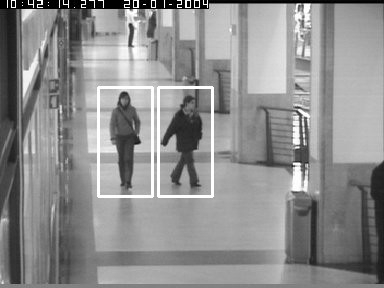
\includegraphics[width=11cm]{Obrazy/person-detection.png}
        \caption{Przykład rozpoznawania osób na obrazie~\cite{rozpoznawanieObiektow}.}
        \label{fig.rozpoznawanieObiektow}
    \end{figure}

    Można znaleźć wiele witryn internetowych, które udostępniają interfejsy programistyczne umożliwiające zaimplementowanie
    rozpoznawania wieku z obrazu.
    Istnieją algorytmy przetwarzania obrazu, które oprócz wieku wyznaczają z pewnym prawdopodobieństwem płeć danej osoby.
    Oprócz płci mogą one także wyznaczyć emocję oraz czy dana osoba nosi okulary.

    Z weryfikacją wieku danej osoby można się spotkać przed wejściem do niektórych miejsc, takich jak
    klub nocny.
    Większość osób
    musi okazać ważny dowód osobisty,
    co generuje duże kolejki do wejścia.
    Aplikacje analizujące wiek na podstawie obrazu twarzy z kamery przed wejściem
    do takich miejsc znacząco usprawniłyby weryfikację wieku.
    Rozpoznawanie wieku może być wykorzystywane przy analizie średniego wieku ludzi w jakimś miejscu np.
    podczas demonstracji.

    Wiele gier posiada treści nieodpowiednie dla młodszych użytkowników.
    Możliwe jest stosowanie technologii wykrywania
    wieku użytkownika przed udostępnieniem mu treści, która wymaga odpowiedniego wieku.

    Można znaleźć o wiele więcej potencjalnych zastosowań przetwarzania obrazu oraz rozpoznawania wieku na podstawie
    tekstury (obrazu) twarzy.
    Z biegiem lat z pewnością będzie można zauważyć dalszy rozwój tej dziedziny, która
    opiera się w głównej mierze na sztucznej inteligencji~\cite{computerVision}.
    %275 wyrazow
    \section*{Cel i zakres pracy}\label{sec:cel-i-zakres-pracy}
    %    Celem pracy magisterskiej jest stworzenie prostego programu do rozpoznawania wieku na podstawie tekstury twarzy.
    %
    %    Zakres pracy obejmuje:
    %    \begin{itemize}
    %        \item Wybór bazowej metody wyznaczania wieku
    %        \item Stworzenie kilku modyfikacji bazowej metody
    %        \item Opis algorytmów każdej z metod wyznaczania wieku
    %        \item Porównanie wszystkich metod i wybór najlepszej
    %    \end{itemize}
    %
    %    \chapter{Przegląd metod wyznaczania wieku}
    %    \section{Metoda a}
    %    \section{Metoda b}
    %    \section{Metoda wrinkle feature}
    Celem niniejszej pracy jest stworzenie algorytmu do szacowania wieku.
    Bazą dla przeprowadzonych badań było odtworzenie pracy ,,Age Estimation from Face Image using Wrinkle
    Features''~\cite{wrinkleFeatures}. Metodę w niej zawartą poddano następnie kilku modyfikacjom.

    Zakres pracy obejmuje następujące zagadnienia:
    \begin{itemize}
        \item Implementacja algorytmu z pracy~\cite{wrinkleFeatures}, w dalszej części pracy określanego jako metoda
        oryginalna lub metoda bazowa;
        \item Zaproponowanie kilku modyfikacji oryginalnej metody;
        \item Opis algorytmów oraz zmian w stosunku do oryginalnej metody;
        \item Przeprowadzenie badań w celu rozstrzygnięcia, który algorytm jest najskuteczniejszy w działaniu;
        \item Wyciągnięcie wniosków z przeprowadzonych badań.
    \end{itemize}
    W rozdziale~\ref{ch:metoda-bazowa---wrinkle-feature} zaprezentowano algorytm szacowania wieku oparty na oryginalnej metodzie.
    W pierwszej sekcji~\ref{sec:metodaWykrywaniaTwarzy} skupiono się na metodach wykrywania twarzy wraz z opisem
    metody wykrywania w bazowym algorytmie.
    Następnie w sekcji~\ref{sec:wyznaczanieStref} zaprezentowano sposób wyznaczania stref zmarszczkowych z oryginalnej metody.
    W kolejnej sekcji~\ref{sec:wykrywanie-zmarszczek---detektor-canny} przedstawiono sposób detekcji zmarszczek na twarzy implementowany
    w metodzie bazowej.
    Przedostatnia sekcja rozdziału drugiego~\ref{sec:algorytmTrenowania}  prezentuje sposób analizy % w pracy
    zależności pomiędzy wskaźnikiem zmarszczek, a wiekiem
    danej osoby.
    W ostatniej sekcji~\ref{sec:grupowanieDanych} tego rozdziału przedstawiono algorytm grupowania danych niezbędny do oszacowania wieku.

    W kolejnym rozdziale~\ref{ch:modyfikacje-metody-bazowej} opisuje 3 modyfikację oryginalnej metody.
    Oprócz sposobu implementacji danych modyfikacji czytelnik zostaje zapoznany z teoretycznymi podstawami wykrywania zmarszczek za
    pomocą metody HOG (ang. Histogram of Oriented Gradients) oraz szacowania wieku dzięki algorytmowi KNN (ang.  k-nearest neighbors).

    W przedostatnim rozdziale~\ref{ch:badania} przedstawiono sposób realizacji badań oraz ich wyniki.
    W ostatnim rozdziale~\ref{ch:podsumowanie} podsumowano niniejsza pracą.

    \chapter{Metoda bazowa - wskaźnik zmarszczek}\label{ch:metoda-bazowa---wrinkle-feature}

    Istnieje wiele metod wyznaczania wieku z obrazu twarzy.
    Jedna z pierwszych metod szacowania wieku opierała się na wyznaczaniu proporcji twarzy, a następnie na detekcji i
    interpretacji zmarszczek.
    Była ona w stanie ze stuprocentową poprawnością wyznaczyć, czy dana osoba jest osobą
    dorosłą, czy
    dzieckiem~\cite{kwonLobo}.

    W kolejnych latach algorytmy i techniki szacowania wieku były udoskonalane.
    Badano wpływ starzenia się osób na
    wygląd skóry.
    Oprócz naturalnych
    zmian skóry pod wpływem jej starzenia sie należało uwzględnić także inne
    czynniki, do których należą między innymi
    płeć, poziom stresu, czy ekspozycja na działanie środowiska zewnętrznego.
    Badania tego rodzaju opisano w pracy~\cite{lanitisTaylor} A. Lanitis, Ch. J. Taylor oraz T. F. Cootes.
    Ponadto w tej pracy zaprezentowano algorytm rozpoznawania płci, emocji czy osób na podstawie obrazu twarzy.

    W kolejnych latach zaczęto przeprowadzać porównania cech twarzy tej samej osoby w różnym wieku.
    Różnice w powyższych cechach posłużyły do zbudowania statystyki zmian cech twarzy wraz ze starzeniem się.
    Taka analiza została zaprezentowana w pracy~\cite{ramanthanChelappa} N. Ramanathan oraz R. Chellappa.
    Rozwinięciem tego pomysłu była praca~\cite{gengZhou} X. Geng, Z. Zhou i K. Smith-Miles.
    W tym artykule porównywano sekwencje wielu zdjęć twarzy jednej osoby.
    Zdjęcia przestawiały twarz w różnym wieku.
    Te badania pozwoliły na zbudowanie wzorca starzenia się twarzy.
    Z kolei M.M. Dehshibi oraz A. Bastanfard w swojej pracy~\cite{dehshibiBastard} analizują proporcje twarzy oraz ilość
    zmarszczek przy szacowaniu wieku.
    Praca~\cite{khryashchevGanin} autorstwa
    Vladimira Khryashcheva, Alexandra Ganina, Olgi Stepanovej oraz
    Antona Lebedeva zawiera podsumowanie technik szacowania wieku.
    Wynika z niego, że do wyodrębniania cech z twarzy stosuje się BIF(ang. biologically inspired features).
    Powyższa metoda została zaprezentowana w książce~\cite{bif} Guodong Guo i in.
    Mniej popularne metody analizujące cechy twarzy to filtry Gabora oraz LBP (ang. local binary patterns)~\cite{lbp}.


    W metodzie bazowej, która została opisana w artykule~\cite{wrinkleFeatures}, wykrywanie wieku dzieli się na kilka
    faz.
    Na początku należy wykryć twarz.
    Zastosowany algorytm wykrywania został
    opisany w sekcji~\ref{sec:metodaWykrywaniaTwarzy}.
    Następnie należy wyznaczyć strefy zmarszczkowe na twarzy.
    W artykule~\cite{wrinkleFeatures} udowodniono,
    że istnieje kilka konkretnych stref, w których następuje znacząca zmiana ilości zmarszczek wraz z wiekiem.
    Powyższe strefy zostały wymienione w sekcji~\ref{sec:wyznaczanieStref}.
    Sekcja~\ref{sec:wykrywanie-zmarszczek---detektor-canny} przedstawia technikę
    wykrywania zmarszczek znajdujących się w strefach.
    Wykryte zmarszczki
    pozwalają na obliczenie wskaźnika zmarszczek dla danej twarzy, zgodnie z opisem w sekcji~\ref{sec:wyliczanieWrinkleFeature}.
    W tym miejscu kończy się faza wyznaczania wskaźnika zmarszczek dla danej osoby (rysunek~\ref{fig.faza1Algorytmu}).
    Kolejna faza
    jest potrzebna do
    znalezienia relacji pomiędzy wskaźnikiem zmarszczek a wiekiem.
    Do tego celu należy zastosować algorytm trenujący, który
    został opisany w sekcji~\ref{sec:algorytmTrenowania}.
    Wynikiem algorytmu trenującego jest zbiór danych, który
    należy pogrupować, tak jak to opisano w sekcji~\ref{sec:grupowanieDanych}.
    Ostatnią fazą algorytmu jest wykrywanie wieku
    na podstawie wyników działania FCM (ang. Fuzzy C-Means) - sekcja~\ref{sec:grupowanieDanych}
    (rysunek~\ref{fig .faza2Algorytmu}).

    \begin{figure}[ht!]
        \centering
        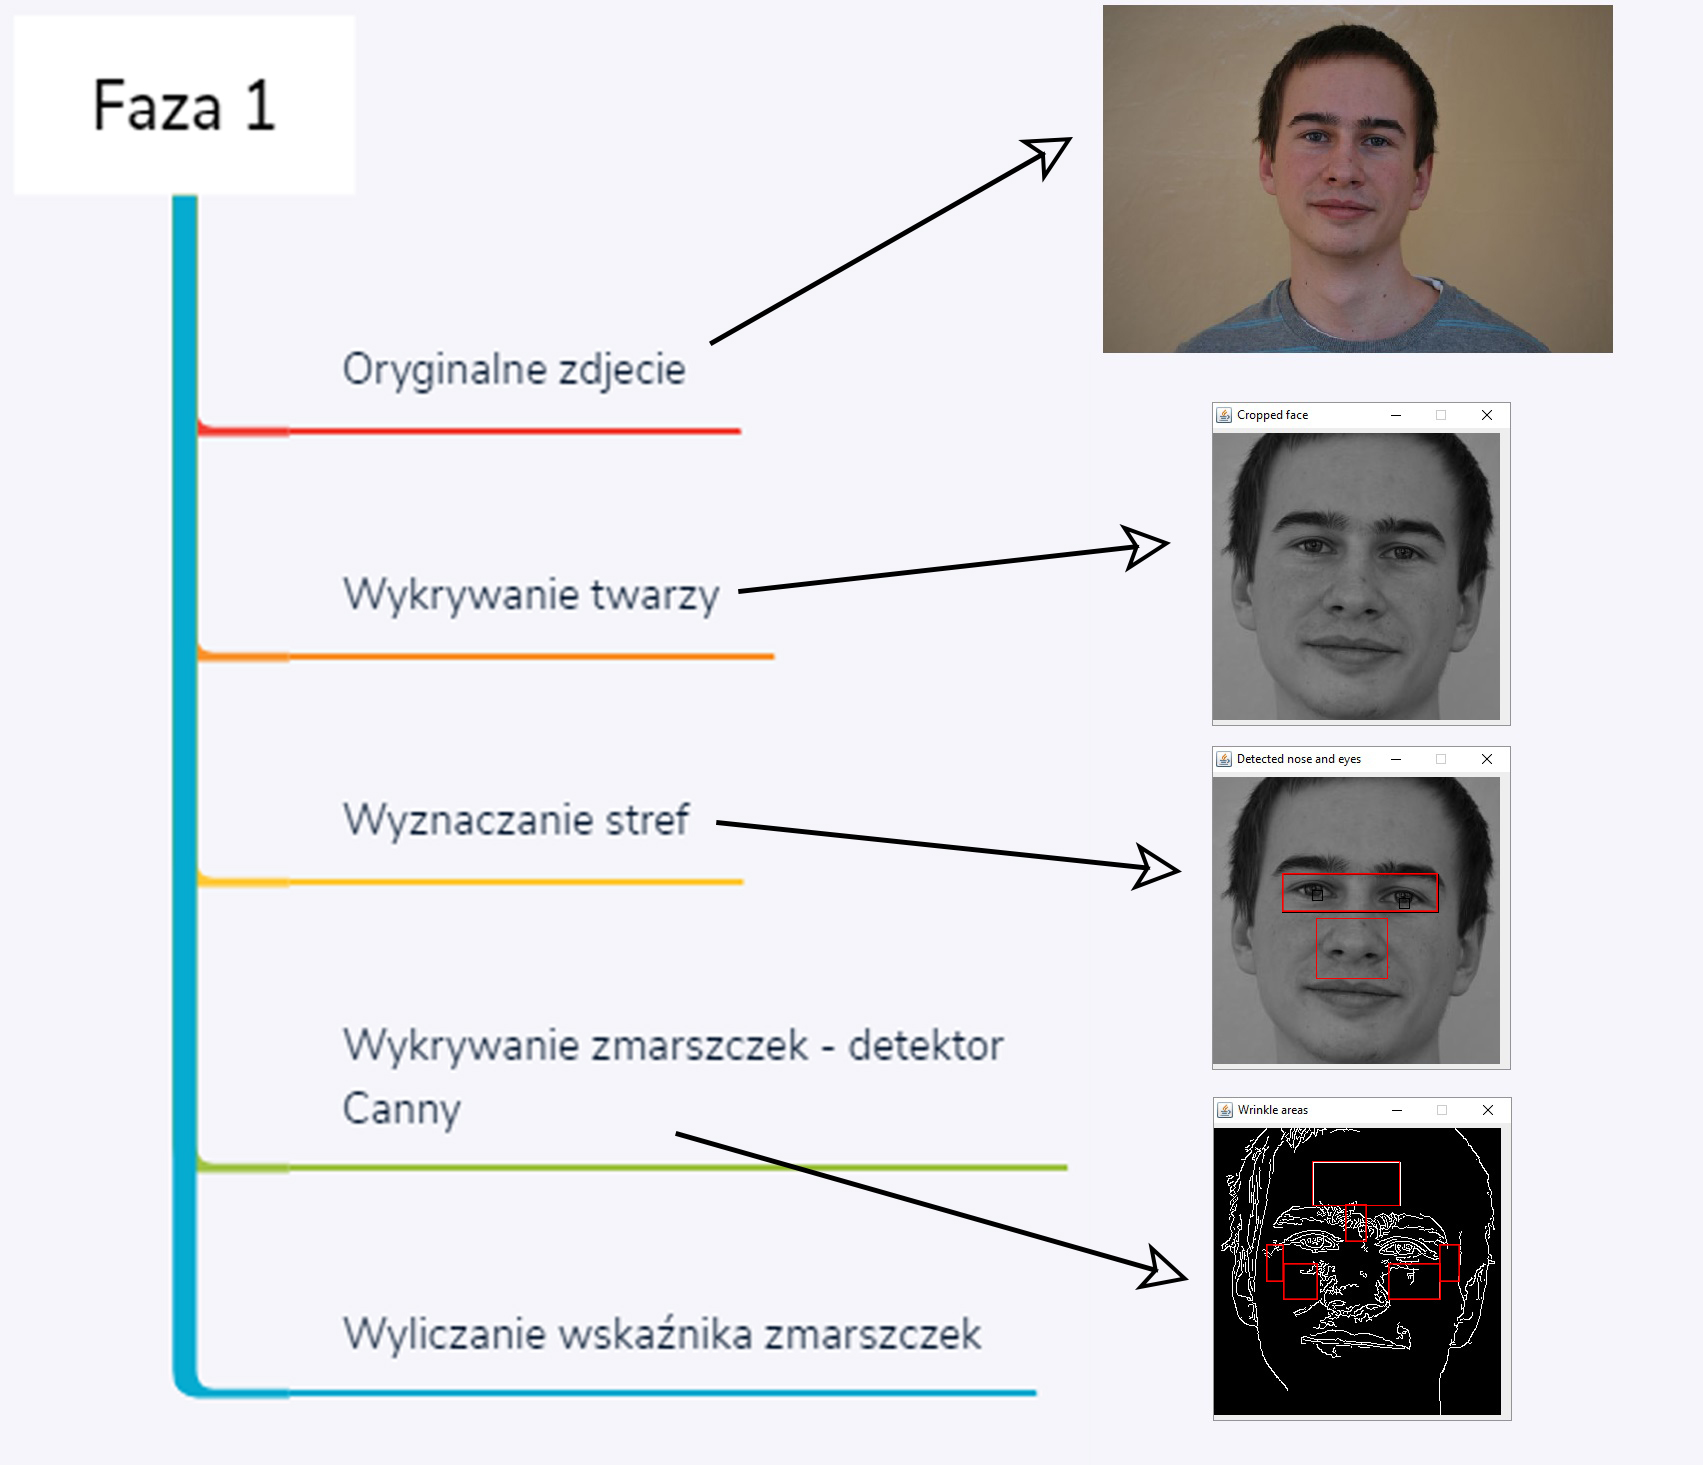
\includegraphics[width=12cm]{Obrazy/Faza1.jpg}
        \caption{Faza 1 algorytmu}
        \label{fig.faza1Algorytmu}
    \end{figure}

    \begin{figure}[ht!]
        \centering
        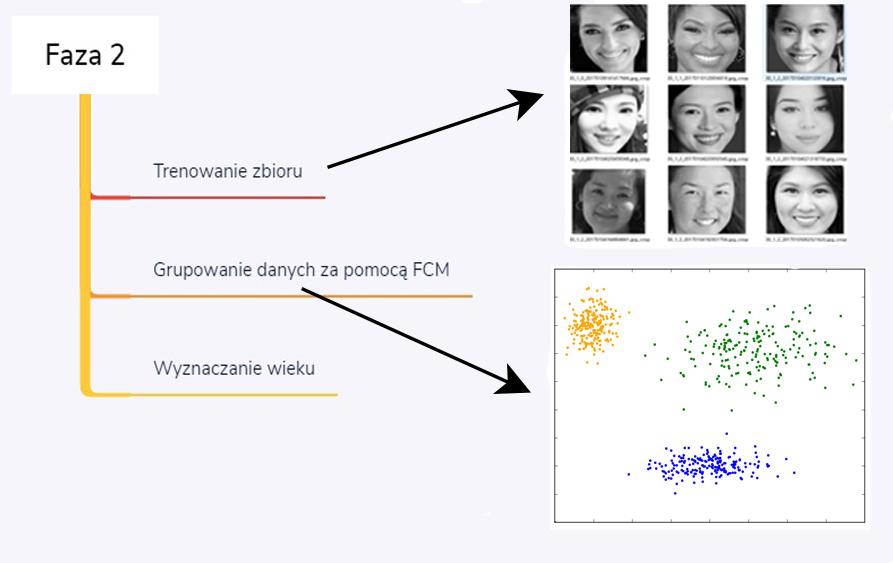
\includegraphics[width=12cm]{Obrazy/Faza2.jpg}
        \caption{Faza 2 algorytmu}
        \label{fig.faza2Algorytmu}
    \end{figure}

    \clearpage
    \section{Metoda wykrywania twarzy}\label{sec:metodaWykrywaniaTwarzy}
    W literaturze można odnaleźć wiele metod wykrywania twarzy.
    Istnieje kilka podejść aby skutecznie wykrywać twarz na danym obrazie~\cite{mehdiRizvi}:
    %       https://www.researchgate.net/publication/257338580_A_Review_on_Face_Detection_Methods
    %     Knowledge-based methods: These rule-based methods encode human knowledge
    %    of what constitutes a typical face. Usually, the rules capture the relationships
    %    between facial features. These methods are designed mainly for face localization.
    %     Feature invariant approaches: These algorithms aim to find structural features that
    %    exist even when the pose, viewpoint, or lighting conditions vary, and then use these
    %    to locate faces. These methods are designed mainly for face localization.
    %     Template matching methods: Several standard patterns of a face are stored to
    %    describe the face as a whole or the facial features separately. The correlations
    %    between an input image and the stored patterns are computed for detection. These
    %    methods have been used for both face localization and detection.
    %     Appearance-based methods: In contrast to template matching, the models (or
    %    templates) are learned from a set of training images which should capture the
    %    representative variability of facial appearance. These learned models are then used
    %    for detection. These methods are designed mainly for face detection.

    \begin{itemize}
        \item metoda oparta na nauce (ang. knowledge - based method):

        Metoda oparta na nauce kieruje się wiedzą na temat wyglądu twarzy, a
        bardziej precyzyjnie chodzi o charakterystyczne cechy,
        dzięki którym na zdjęciu można wyodrębnić obszar twarzy.
        Mowa tutaj o cechach takich jak kształt twarzy, kolor, miejsca o różnej jasności czy specyficzne krawędzie
        tworzone np. przez
        usta.
        \item metoda niezmienności cech (ang. features invariant method):

        W metodzie niezmienności cech wyszukuje się strukturalne cechy twarzy, które są widoczne w każdych warunkach
        oświetleniowych.
        Ponadto te cechy są widoczne bez względu na punkt widzenia, nawet jeśli twarz jest przedstawiona
        z profilu czy przechylona pod kątem.
        \item metoda dopasowania szablonu twarzy (ang. template matching method):

        Metoda dopasowania szablonu twarzy wykorzystuje kilka standardowych wzorów opisujących twarz.
        Na wejściu algorytmu obraz jest porównywany z tymi wzorami, a
        na wyjściu dostajemy informację, w jakim stopniu obraz jest dopasowany do ogólnego szablonu twarzy.
        \item metoda bazująca na wyglądzie (ang. appearance - based method):

        Ideą metody bazującej na wyglądzie jest analiza dużego zbioru obrazów twarzy, tak aby wychwycić zmienność
        ich cech.
        Tak wytrenowany model jest później wykorzystywany do wykrywania twarzy.
    \end{itemize}

    %       https://www.researchgate.net/publication/257338580_A_Review_on_Face_Detection_Methods
    %    Pose: The images of a face vary due to the relative camera-face pose (frontal, 45
    %    degree, profile, upside down), and some facial features such as an eye or the nose
    %    may become partially or wholly occluded.
    %     Presence or absence of structural components: Facial features such as beards,
    %    mustaches, and glasses may or may not be present and there is a great deal of
    %    variability among these components including shape, color, and size.
    %     Facial expression: The appearance of faces is directly affected by a person’s facial
    %    expression.
    %     Occlusion: Faces may be partially occluded by other objects. In an image with a
    %    group of people, some faces may partially occlude other faces.
    %     Image orientation: Face images directly vary for different rotations about the
    %    camera’s optical axis.
    %     Imaging conditions: When the image is formed, factors such as lighting (spectra,
    %    source distribution and intensity) and camera characteristics (sensor response,
    %    lenses) affect the appearance of a face.
    %    Każda z nich wyodrębnia z obrazu pewne cechy, które
    %    mogą wskazywać, że na danym obszarze obrazu znajduje się twarz.

    Należy jednak zauważyć, że w procesie ekstrakcji twarzy z obrazu mogą wystąpić liczne problemy.~\cite{mehdiRizvi}.
    Jednym z nich jest nieodpowiednia poza.
    Wiąże się to z różnymi ustawieniami twarzy wobec aparatu fotograficznego lub kamery.
    Twarz może być nachylona, przechylona lub odchylona.
    Inaczej mówiąc, może mieć różne położenie w trzech wymiarach, a
    niektóre części twarzy lub jej cechy mogą zostać przysłonięte.
    Im mniej cech widocznych na twarzy, tym mniej danych, które algorytm może z niej wyodrębnić, a
    im mniej danych, którymi algorytm operuje, tym mniejsze prawdopodobieństwo prawidłowego wykrycia twarzy.
    Niektóre twarze mogą zawierać pewne wyróżniające je cechy takie jak broda, blizny czy okulary.
    Różnorodność tych cech także wpływa na efektywność wykrywania twarzy.

    Zdarza się, że twarz zostaje częściowo przysłonięta przez jakiś inny obiekt.
    Na przykład na zdjęciu,
    które obejmuje grupę wielu osób, część danej twarzy może być przysłonięta przez inną twarz.
    Takie przysłonięcie przez inny obiekt wiąże się z utratą informacji o części twarzy, co zmniejsza prawdopodobieństwo
    prawidłowego jej wykrycia.

    Ilość zmarszczek na twarzy jest zmienna, w zależności od wyrazu mimicznego.
    Przy różnych minach zmienia się kształt ust, a czasem w wyniku pracy mięśni uwydatniają się na twarzy ostre
    krawędzie.
    Widoczne mogą być różne pofałdowania skóry.

    Kolejnym istotnym elementem jest oświetlenie twarzy.
    Gdy twarz oświetlona jest tzw. ostrym światłem, występują na
    niej cienie i światła określane jako ostre (obraz~\ref{fig.oswietlenieTwarzy}).
    \begin{figure}[h!]
        \centering
        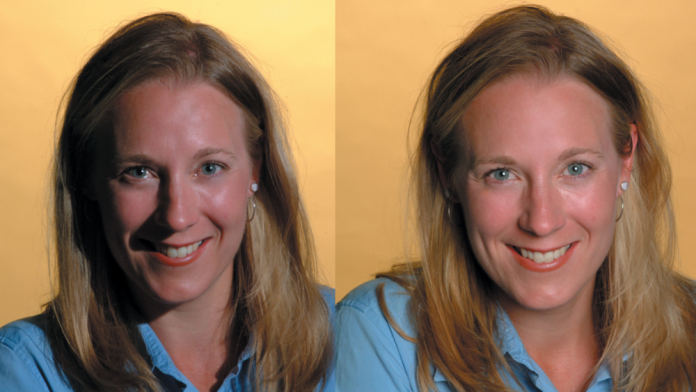
\includegraphics[width=12cm]{Obrazy/oswietlenieTwarzy.jpg}
        \caption{Przykład twarzy oświetlonej ostrym (twarz po lewej) oraz miękkim światłem~\cite{oswietlenieTwarzy}.}
        \label{fig.oswietlenieTwarzy}
    \end{figure}
    W tym przypadku ryzyko utraty szczegółów oświetlanej twarzy jest większe.
    Kiedy twarz jest skierowana na wprost słońca, z dużym
    prawdopodobieństwem można stwierdzić, że zostanie oświetlona ostrym światłem.
    Z kolei miękkie światło jest generowane na przykład przez zachmurzone niebo.
    Istotne jest także źródło światła, które
    może być punktowe lub rozproszone.
    Przy punktowym źródle światła cała twarz jest
    okryta jednolitym cieniem, którego intensywność zależy od rodzaju światła.
    Natomiast przy świetle rozproszonym intensywność cieni jest mniejsza.
    Na rys.~\ref{fig.technikiWykrywaniaTwarzy} przedstawione są różne techniki wykrywania twarzy.
    \begin{figure}
        \centering
        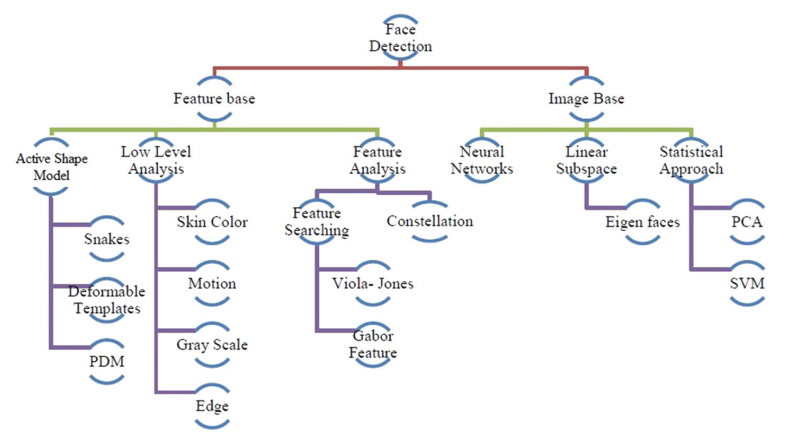
\includegraphics[width=15cm]{Obrazy/technikiWykrywaniaTwarzy.jpg}
        \caption{Różne techniki wykrywania twarzy~\cite{faceDetectionTechniques}.}
        \label{fig.technikiWykrywaniaTwarzy}
    \end{figure}
    %    https://sci-hub.tw/10.1007/s10462-018-9650-2

    %    Wyodrębnianie lub ekstrakcja cech polega na przekształceniu obrazu do zbioru zmiennych, które
    %    zostaną później użyte w wykrywaniu obiektu lub obiektów na obrazie.

    Jak widać metod wykrywania twarzy jest sporo,
    a szczegółowe omówienie każdej z nich nie byłoby merytorycznie uzasadnione.
    Poniżej zostaną przytoczone dwie metody wykrywania twarzy.
    Dodatkowo zostanie omówiona metoda, która posłużyła do wykrywania twarzy w niniejszej pracy.

    %https://sci-hub.tw/10.1016/S0031-3203(00)00134-5
    W pracy~\cite{wongLamSiu}
    przedstawiono opisaną w skrócie poniżej technikę wykrywania twarzy.
    W pierwszym etapie procesu obszary, gdzie może znajdować się ludzkie oko,
    są wykrywane przez przeprowadzenie testów na zacienionych rejonach obrazu.
    Pary takich obszarów wyodrębnia się na podstawie algorytmu genetycznego,
    aby następnie wyznaczyć możliwy obszar twarzy.
    Dla każdego obszaru mierzy się wartość dopasowania na podstawie jego projekcji na wektory własne, obliczone dla
    obszarów twarzy, tzw. eigenfaces.
    Aby wiarygodność wykrywania była wyższa,
    każdy możliwy obszar twarzy normalizuje się pod kątem oświetlenia.
    Proces ten powtarza się pewną ilość razy,
    a następnie do dalszej weryfikacji są wybierane możliwe obszary twarzy o wysokiej wartości dopasowania.
    Na tym etapie mierzy się symetrię twarzy oraz sprawdza się,
    czy na każdym wybranym obszarze istnieją rysy twarzy.
    Rysy określa się przez ewaluację rzeźby topograficznej - wystających i wklęsłych elementów
    różnych regionów obszaru twarzy, poddanego uprzednio normalizacji.
    Algorytm jest w stanie wykryć obszar twarzy także wtedy, gdy głowa jest przechylona.

    %Druga metoda wykrywania twarzy z https://www.researchgate.net/publication/334770252_An_Accurate_System_for_Face_Detection_and_Recognition
    %https://sci-hub.tw/10.1007/s10462-018-9650-2
    W roku 1997 w pracy~\cite{clowleyCoutaz} opisano metodę wykrywania twarzy bazującą na
    wykrywaniu cechy, jaką jest kolor skóry.
    Zarówno dla człowieka, jak i dla maszyny kolor skóry jest
    najbardziej widoczną cechą twarzy.
    Ponadto kolor jest przetwarzany znacznie szybciej niż inne cechy.
    Przy dobrych warunkach oświetleniowych ustawienie twarzy nie ma wpływu na skuteczność wykrywalności twarzy
    opisywaną metodą.

    Niezależnie od wybranej metody mogą wystąpić problemy z poprawnym wykryciem twarzy.
    Jednym z nich jest problem wykrywalności twarzy przy nierównomiernym oświetleniu.
    Problem pojawia się także, gdy na obrazie widoczny jest obszar skóry spoza twarzy, np. z rąk.
    Warto zaznaczyć, że kolor twarzy na obrazie jest zależny od względnego kierunku oświetlenia.
    Obszar twarzy w omawianym algorytmie jest wykrywany poprzez normalizacje histogramu kolorów.
    Normalizacja jest potrzebna do redukcji wpływu natężenia oświetlenia na kolor.

    %trzecia metoda  - wstep do Haar Cascade https://drive.google.com/file/d/1nJ9S3HtuuFY6O1FLdIjRWSzWUFwZ_fuJ/view?usp=sharing
    Algorytm Haar Cascade jest jedynym algorytmem do wykrywania twarzy zaimplementowanym w bibliotece OpenCV,
    dlatego został wykorzystany w procesie badawczym.
    Algorytm został bliżej przedstawiony w książce~\cite{violaJones} w 2001 roku i składa się z trzech podstawowych faz,
    których dokładny opis znajduje sie w sekcji~\ref{subsec:algorytm-haar-cascade}.
    %    W pierwszej obraz wejściowy przekształcany jest na obraz scałkowany.
    %    Następnie wykorzystywany jest algorytm do boostingu, który zmniejsza ilość klasyfikatorów tylko do tych
    %    najbardziej istotnych.
    %    W ostatniej fazie klasyfikatory łączone są w kaskady w celu przyspieszenia procesu wykrywania twarzy.
    %    Znaczna większość metod wykrywania obiektów na obrazie (w tym twarzy) wymaga wstępnego przekształcenia obrazu do
    %    skali szarości.
    %

    %    https://towardsdatascience.com/face-recognition-with-opencv-haar-cascade-a289b6ff042a
    %    przez kogo został zaproponowany...
    %    byc moze cos o funkcji kaskadowej
    %    o tym ze OpenCv zawiera wytrenowane algorytmy Haar Cascade ktore wykrywaja ryj, oczy, usta itp
    %    wkleic obrazek z rodzajami filtrow
    %    jak dziala ten filtr
    %    przyklad na gebie emmy watson moze...
    %cosik tam jeszcze

    %    opisac jak dokladnie zaimplementowano to u nas
    %    przejscie na skale szarosci podczas wykrywania... czym ona jest?...
    \subsection{Przestrzenie barw oraz skala szarości}\label{subsec:konwersja-do-skali-szarości-oraz-przestrzenie-barw}
    %https://sci-hub.tw/10.1007/s10462-018-9650-2
    Każdy piksel w trybie kolorowym ma określoną reprezentację barwy z określonego modelu.
    Najczęściej są to trzy lub cztery
    wartości~\cite{przestrzenieKolorow}.
    Do przestrzeni barw zaliczają się:
    \begin{itemize}
        \item CIEXYZ,
        \item CMYK,
        \item RGB.
    \end{itemize}

    W dziedzinie rozpoznawania obrazów najczęściej barwy są reprezentowane przez przestrzeń barw
    RGB~\cite{przestrzenieKolorow}.
    Przestrzeń kolorów RGB składa się z trzech kanałów~\cite{kolory}:
    \begin{itemize}
        \item R - czerwonego (z ang. Red),
        \item G - zielonego (z ang. Green),
        \item B - niebieskiego (z ang. Blue).
    \end{itemize}
    Barwy mieszane są poprzez syntezę addytywną.
    W przeciwieństwie do syntezy subtraktywnej, barwa wynikowa powstaje tu poprzez sumowanie wiązek światła widzialnego o
    różnych długościach~\cite{przestrzenieKolorow}.
    Każdy piksel opisany za pomocą przestrzeni barw RGB ma trzy 8-bitowe wartości reprezentujące każdy kanał.
    Spotykane
    są 12- lub 16-bitowe reprezentacje kanałów, jednak 8-bitowa jest najpopularniejsza.
    Dla 8-bitowych kanałów
    wartość ,,0''
    danego kanału oznacza brak jasności, natomiast ,,255'' maksymalną jasność.
    Poprzez mieszanie jasności tych trzech kanałów
    można uzyskać szerokie spektrum barw (rysunek~\ref{fig.mieszanieKolorow}).

    \begin{figure}[h!]
        \centering
        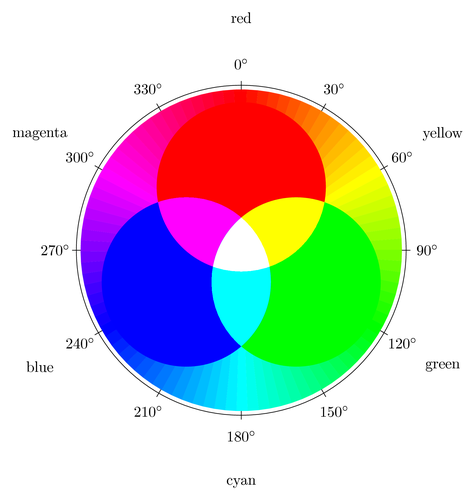
\includegraphics[width=7cm]{Obrazy/mieszanieKolorow.jpg}
        \caption{Mieszanie kanałów RGB~\cite{colorMixing}.}
        \label{fig.mieszanieKolorow}
    \end{figure}

    Przykładowo kolor o reprezentacji R=153, G=217, B=234 przedstawiono na rysunku~\ref{fig.mieszanieKolorowBlekitny}

    \begin{figure}
        \centering
        
\includegraphics[width=2cm]{Obrazy/blekitny.jpg}
        \caption{Kolor R=153 G=217 B=234.}
        \label{fig.mieszanieKolorowBlekitny}
    \end{figure}

    Kolor (rysunek~\ref{fig.mieszanieKolorowBlekitny}) może być też reprezentowany w kodzie szesnastkowym \#99D9EA.
    Każda
    wartość heksadecymalna odpowiada kolejno kanałowi R, G, B.

    Obraz może też być przedstawiony za pomocą odcieni jednej barwy.
    Taki obraz nazywa się obrazem monochromatycznym.
    Najczęściej stosowaną barwą w takich obrazach jest szarość~\cite{przestrzenieKolorow}.

    Istnieją 3 metody konwersji obrazu z przestrzeni RGB na monochromatyczny~\cite{colorMixing}:
    \begin{itemize}
        \item największej jasności,
        \item średnia,
        \item luminancji.
    \end{itemize}
    Metoda największej jasności konwertuje na skalę szarości wg wzoru~\ref{wzor.najwiekszaJasnosc}.

    \large
    \begin{equation}
        \frac{(max(R, G, B) + min(R, G, B))}{2}
        \label{wzor.najwiekszaJasnosc}
    \end{equation}
    \normalsize
    Metoda średnia bazuje na wzorze~\ref{wzor.metodaSrednia}, natomiast metodę luminancji ilustruje wzór~\ref{wzor.metodaLuminancji}.

    \large
    \begin{equation}
        \frac{(R + G + B)}{3}
        \label{wzor.metodaSrednia}
    \end{equation}
    \normalsize

    \large
    \begin{equation}
        0,21 R + 0,72 G + 0,07 B
        \label{wzor.metodaLuminancji}
    \end{equation}
    \normalsize

    W pracy zastosowano konwersję z przestrzeni RGB na skale szarości wg wzoru~\ref{wzor.rgb2grayopencv}
    zaimplementowanego w bibliotece OpenCV, który jest modyfikacją metody luminancji.

    \large
    \begin{equation}
        0,299 R + 0,587 G + 0,114 B
        \label{wzor.rgb2grayopencv}
    \end{equation}
    \normalsize

    \subsection{Metoda detekcji twarzy}\label{subsec:algorytm-haar-cascade}

    Haar Cascade jest algorytmem służącym do wykrywania obiektów na obrazach.
    Został stworzony przez Paula Violę oraz Michaela Jonesa w 2001 roku~\cite{violaJones}.
    Opiera się na zbudowaniu kaskadowej funkcji za pomocą analizy wielu zdjęć twarzy.
    Obrazy są dzielone na
    dwie kategorie - pozytywne oraz negatywne.
    Na zdjęciach klasyfikowanych jako pozytywne istnieje obiekt, który ma zostać wykryty, natomiast
    na zdjęciach negatywnych nie ma tego obiektu.
    Ekstrakcja cech w algorytmie Violi i Jonesa jest realizowana przez filtry Haara.
    %    Są to prostokątne okienka
    %    nakładane na obraz, które analizują jasność pikseli (rysunek~\ref{fig.haarRectangles}).
    Przed zastosowaniem filtru obraz musi zostać przekształcony do skali szarości.
    Filtry mają postać białych i czarnych prostokątów pogrupowanych w okna (rysunek~\ref{fig.haarRectangles}).
    \begin{figure}
        \centering
        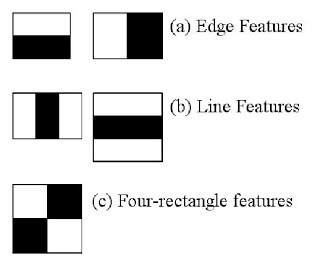
\includegraphics[width=7cm]{Obrazy/Haar_filter_rectangles.jpg}
        \caption{Filtr Haara a) krawędziowy b) liniowy c) szachownica~\cite{haar}}
        \label{fig.haarRectangles}
    \end{figure}
    Wyznaczana jest suma jasności pikseli w obu rodzajach prostokątów, a
    następnie dla każdego okna obliczana jest różnica pomiędzy białymi a czarnymi.
    Na krawędzi istnieje różnica w jasności pikseli, dlatego opisywany algorytm ma zastosowanie w ich wykrywaniu.
    (rysunek~\ref{fig.haarEmmaWatson}).

    \begin{figure}
        \centering
        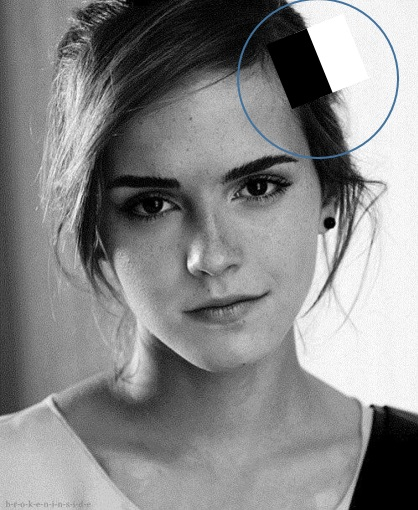
\includegraphics[width=6cm]{Obrazy/haarEmmaWatson.jpg}
        \caption{Filtr Haara nałożony na krawędź twarzy~\cite{haar}}
        \label{fig.haarEmmaWatson}
    \end{figure}

    W celu poprawy efektywności sumowania pikseli stosowane są
    rozwiązania zwane w literaturze obrazem scałkowanym (ang. Integral image lub summed-area table)
    ~\cite{computerVision}.
    Jego ideą jest, aby każdy obraz został przekształcony w
    tabelę, w której każdy element x, y tej tabeli odpowiada sumie jasności wszystkich pikseli według
    wzoru~\ref{wzor.summedAreaTable}.

    \large
    \begin{equation}
        I(x,y) = \sum_{{x}'\leq x \cap {y}'\leq y}^{} i({x}',{y}')
        \label{wzor.summedAreaTable}
    \end{equation}
    \normalsize
    gdzie I(x,y) jest wartością na pozycji x,y w tabeli(tabela obrazu scałkowanego), natomiast i(x,y) oznacza jasność piksela o
    współrzędnych x,y na obrazie.
    Na rysunku~\ref{fig.poiprzedCalkowaniem} przedstawiona jest tabela prezentująca jasność pikseli przed i po
    zastosowaniu całkowania obrazu.
    \begin{figure}
        \centering
        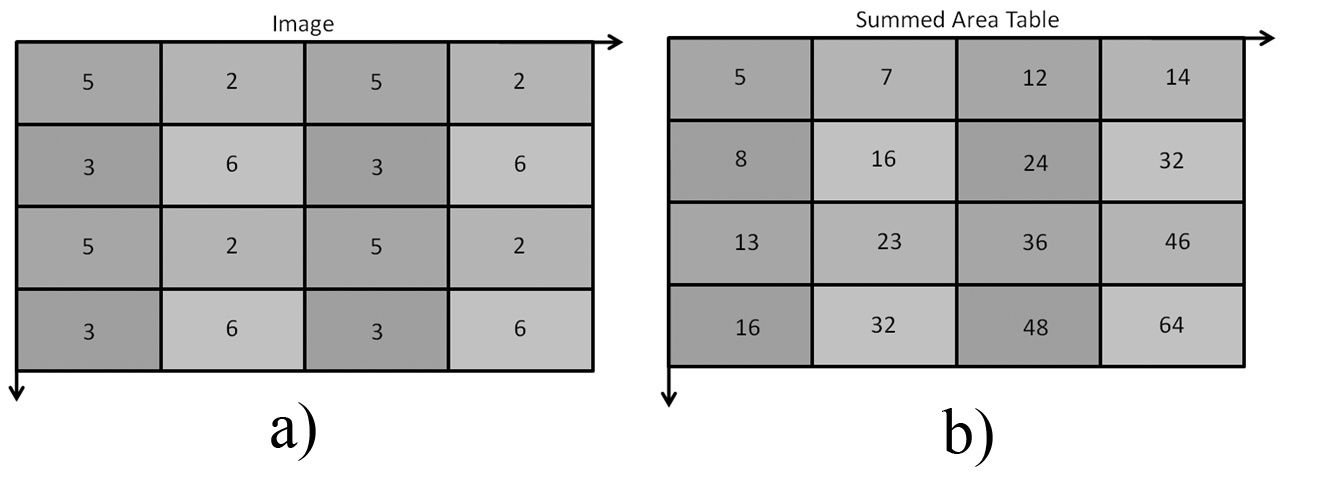
\includegraphics[width=12cm]{Obrazy/poiprzedCalkowaniem.jpg}
        \caption{Tabela jasności poszczególnych pikseli: a) przed zastosowaniem całkowania b) po
        zastosowaniu całkowania~\cite{integralImages}}
        \label{fig.poiprzedCalkowaniem}
    \end{figure}

    Sumowanie przykładowego okna (rysunek~\ref{fig.sumowanieOkna}) wymaga czterech operacji (wzór~\ref{wzor.windowsSum}).
    \begin{figure}
        \centering
        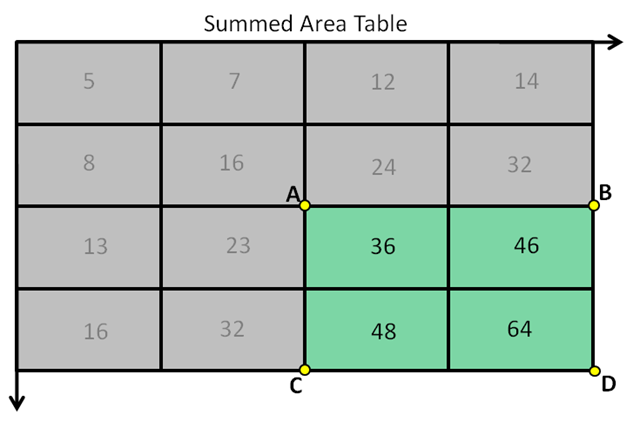
\includegraphics[width=6cm]{Obrazy/sumowanieOkna.jpg}
        \caption{Sumowanie okna~\cite{integralImages}}
        \label{fig.sumowanieOkna}
    \end{figure}


    \large
    \begin{equation}
        \sum_{x_0\leq x \leq x_1\cap {y}\leq y \leq y_1}^{} i(x,y) = I(D) + I(A) - I(B) - I(C)
        \label{wzor.windowsSum}
    \end{equation}
    \normalsize
    gdzie lewa część równania oznacza sumę jasności pikseli
    zaznaczonego okna tj.
    na rysunku~\ref{fig.sumowanieOkna}, I(A) - wartość scałkowanego obrazu przy punkcie A
    (analogicznie I(B), I(C), I(D)) - (rysunek~\ref{fig.sumowanieOkna}).

    W związku z powyższym obliczenie wartości dla krawędziowego filtru Haara wymaga obliczenia różnicy dwóch sum,
    zatem do uzyskania wyniku konieczne jest wykonanie ośmiu operacji.
    Reprezentacja obrazu za pomocą obrazu scałkowanego znacznie zwiększa efektywność obliczania wartości w filtrze
    Haara.

    Liczba cech wykrywanych w danym zdjęciu za
    pomocą filtru Haara jest znacznie większa od liczby pikseli na obrazie~\cite{violaJones}.
    Dla obrazu o wymiarach 24x24 pikseli liczba cech wynosi ponad 180000.
    Autorzy algorytmu stwierdzili, że dla zwiększenia jego szybkości należy wybrać małą grupę istotnych cech,
    które razem mogą stworzyć jeden efektywny klasyfikator obiektu, zwany również silnym klasyfikatorem. Ten
    klasyfikator składa się z wielu słabych klasyfikatorów. Każdy z nich na podstawie jednej istotnej cechy dostarcza
    informacji, czy na obrazie znajduje się twarz, czy nie. Liczba tych
    istotnych cech została ustalona na 2500.
    W celu wyodrębnienia tych istotnych cech zastosowano algorytm Adaboost, który został opisany poniżej.

    Zbiór n obrazów do trenowania można oznaczyć tak jak we wzorze~\ref{wzor.zbiorTrenujacy}:
    \large
    \begin{equation}
        (O_{x_1}, O_{y_1}), (O_{x_2}, O_{y_2}), \ldots, (O_{x_n}, O_{y_n})
        \label{wzor.zbiorTrenujacy}
    \end{equation}
    \normalsize
    $O_{x_1}$ oznacza obraz z bazy treningowej o indeksie $1$, natomiast $O_{y_1}$ określa, czy dany obraz
    przedstawia twarz ($O_{y_1} = 1$), czy nie ($O_{y_1} = 0$). Obraz przestawiający twarz nazywany jest obrazem
    pozytywnym, natomiast obraz negatywny nie przedstawia twarzy.

    Następnym krokiem jest inicjalizacja wag (wzór~\ref{wzor.wagi}).

    \large
    \begin{equation}
        w_{1,i} = \frac{1}{2m}, \frac{1}{2l}
        \label{wzor.wagi}
    \end{equation}
    \normalsize

    Parametr $\frac{1}{2m}$ jest wagą dla zdjęć pozytywnych, a $\frac{1}{2l}$ oznacza wagę dla obrazów negatywnych.
    Parametry m, l oznaczają odpowiednio liczbę negatywnych oraz pozytywnych zdjęć.

    %    dla t = 1, \ldots, T,
    %    gdzie T oznacza
    %    liczbę cech.
    %    D:
    Następnie inicjalizowany jest parametr t oznaczający istotną cechę, natomiast T oznacza liczbę wszystkich takich
    cech na obrazie.
    Dla każdej
    cechy t = 1, \ldots, T, przeprowadzany jest poniższy proces:

    1. Normalizowane są wagi (wzór~\ref{wzor.adaboost1}):
    \large
    \begin{equation}
        w_{t,i} = \frac{w_{t,i}}{\sum_{j=1}^{n}w_{t,j}}
        \label{wzor.adaboost1}
    \end{equation}
    \normalsize
    $w_{t}$ jest rozkładem prawdopodobieństwa

    2. Dla każdej cechy j, trenowany jest klasyfikator $h_{j}$, który używa tylko jednej cechy wyliczonej z filtru Haara.
    Błąd jest liczony następująco (wzór~\ref{wzor.adaboost2}):
    \large
    \begin{equation}
        w_{t}, \epsilon_{j} = \sum_{i}^{}w_{i} \abs{h_{j}(x_{i}) - y_{i}}
        \label{wzor.adaboost2}
    \end{equation}
    \normalsize

    3. Wybierany jest klasyfikator $h_{t}$ z najmniejszym błędem \epsilon_{t}.

    4. Następuje aktualizacja wag (wzór~\ref{wzor.adaboost3}):
    \large
    \begin{equation}
        w_{t+1,i} = w_{t,i}\beta_{t}^{1-e_{i}}
        \label{wzor.adaboost3}
    \end{equation}
    \normalsize
    gdzie $e_{i} = 0$. Jeśli $x_{i}$ jest sklasyfikowane prawidłowo, wtedy $e_{i}=1$,
    w innym wypadku $\beta_{t} = \frac{\epsilon_{t}}{1 - \epsilon_{t}}$.

    Silny klasyfikator $h(x)$ jest opisany równaniem:
    \large
    \begin{equation}
        h(x) = \left\{ \begin{array}{ll}
                           1 & \textrm{gdy $\sum_{t=1}^{T}\alpha_{t}h_{t}(x) >= \frac{1}{2} \sum_{t=1}^{T}\alpha_{t}$}\\
                           0 & \textrm{w przeciwnym wypadku}\\
        \end{array} \right.
        \label{wzor.adaboost4}
    \end{equation}
    \normalsize
    gdzie $\alpha_{t} = \lg \frac{1}{\beta_{t}}$

    Algorytm Adaboost zmniejsza ilość cech Haara z ponad stu tysięcy do kilkuset - do tych najistotniejszych cech.

    Ostatnim etapem jest wytworzenie kaskady klasyfikatorów.
    Zwiększa ona znacznie szybkość wykrywania pożądanego obiektu na obrazie.
    Ideą kaskady jest zgrupowanie klasyfikatorów,
    które powstały w poprzednim procesie - tzw. procesie boostingu.
    Klasyfikatory są grupowane w okna,
    które są połączone ze sobą tak jak na rysunku~\ref{fig.kaskadaHaar}.
    \begin{figure}
        \centering
        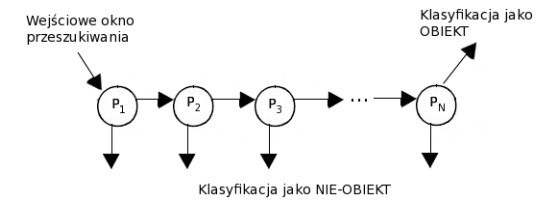
\includegraphics[width=11cm]{Obrazy/kaskadaHaar.jpg}
        \caption{Kaskada klasyfikatorów~\cite{kaskadaHaarObraz}.}
        \label{fig.kaskadaHaar}
    \end{figure}
    Okna są oznaczone jako P1, P2, \ldots, Pn.
    Gdy dane okno wykryje obiekt, przechodzi do kolejnego okna w kaskadzie.
    W przeciwnym wypadku algorytm przerywa działanie i na danym obrazie nie zostaje zidentyfikowany obiekt.
    Okna są poustawiane tak, aby każde z nich klasyfikowało obiekt z różnym prawdopodobieństwem wykrycia oraz
    prawdopodobieństwem błędu.

    Pierwsze okna posiadają klasyfikatory o słabszym TPR oraz FPR niż kolejne.
    Oznacza to, że prawdopodobieństwo TPR w oknie $P_{x-1}$ jest mniejsze od tego w $P_{x}$.
    Natomiast prawdopodobieństwo FPR w oknie $P_{x-1}$ jest większe od tego w $P_{x}$.
    Ostatnie okna mają największy współczynnik TPR oraz najmniejszy FRP ze wszystkich.
    Takie ustawienie okien ma na celu wstępne przepuszczenie przez okna obrazów,
    które z dużym prawdopodobieństwem zawierają szukany obiekt.
    Natomiast ostatnie okna w kaskadzie analizują niewielką część obrazu wejściowego.
    %Opis kaskady
    %    The overall form of the detection process is that of a degenerate decision tree, what we call a “cascade” (see Figure 4). A positive result from the first classifier triggers the
    %    evaluation of a second classifier which has also been adjusted to achieve very high detection rates. A positive result
    %    from the second classifier triggers a third classifier, and so
    %    on. A negative outcome at any point leads to the immediate
    %    rejection of the sub-window.
    %    Stages in the cascade are constructed by training classifiers using AdaBoost and then adjusting the threshold to
    %    minimize false negatives. Note that the default AdaBoost
    %    threshold is designed to yield a low error rate on the training data. In general a lower threshold yields higher de
    %    W ostatniej fazie stosowany jest algorytm kaskady klasyfikatorów.
    %    Klasyfikatory są podzielone na grupy i
    %    połączone ze sobą kaskadowo.
    %    W algorytmie każda grupa może podjąć dwie decyzje - przekazanie danych z klasyfikatorów
    %    do kolejnej grupy lub ich odrzucenie.
    %    Ma to na celu odrzucenie wielu negatywnych danych z klasyfikatorów~\cite{cascade}.

    Biblioteka OpenCV zawiera wytrenowane klasyfikatory, które zostały użyte w tej pracy magisterskiej.
    Wykorzystano
    je do wykrycia twarzy, ust oraz oczu.
    Modele stworzone w wyniku treningu klasyfikatora mają postać plików xml, które można znaleźć na oryginalnym
    repozytorium projektu OpenCv.

    %1600 wyrazow
    \section{Wyznaczanie stref}\label{sec:wyznaczanieStref}
    %Wzory na wyznaczenie stref z "okienek"
    Przed wyznaczeniem stref zmarszczkowych należy zidentyfikować na twarzy oczy oraz nos
    (rysunek~\ref{fig.wykrywanieOczuNosa}).
    \begin{figure}
        \centering
        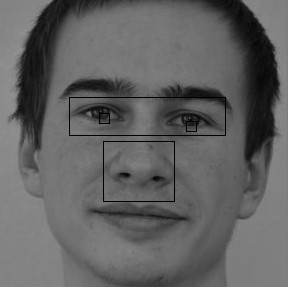
\includegraphics[width=8cm]{Obrazy/wykrywanieOczuNosa.jpg}
        \caption{Wykryty nos oraz oczy.}
        \label{fig.wykrywanieOczuNosa}
    \end{figure}
    Należy podkreślić, że algorytm przerywa działanie jeśli nie zostanie wykryta twarz, oczy lub nos.
    Gdy zostanie wykryty obszar twarzy, oczu oraz nosa wyznaczone zostaje sześć stref zmarszczkowych
    (rysunek~\ref{fig.wykrywanieStrefZmarszczkowych}).

    \begin{figure}
        \centering
        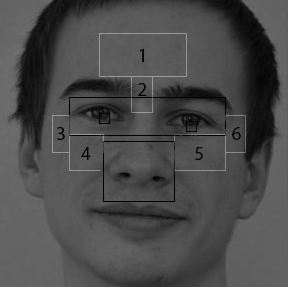
\includegraphics[width=8cm]{Obrazy/strefyZmarszczkowe.jpg}
        \caption{Strefy zmarszczkowe widoczne w białych prostokątach.}
        \label{fig.wykrywanieStrefZmarszczkowych}
    \end{figure}

    Strefy zmarszczkowe są umiejscowione na czole (Strefa ,,1''), w górnej części nosa (Strefa ,,2''), górnej części policzków
    (Strefa ,,4'' i ,,5'') oraz w okolicach powiek (Strefa ,,3'' i ,,6'').
    To właśnie te miejsca zostały uznane przez autorów książki~\cite{wrinkleFeatures} za
    najbardziej znaczące w detekcji wieku.

    Po detekcji oczu należy zmierzyć odległość pomiędzy środkiem lewego oka ($x_{l},y_{l}$),
    a prawego ($x_{p},y_{p}$)
    (wzór~\ref{wzor.odlegloscPomiedzyOczami}).
    \large
    \begin{equation}
        d= \sqrt{\left ( x_{r} - x_{l} \right )^{2}+\left (y_{r} - y_{l}  \right )^{2}}
        \label{wzor.odlegloscPomiedzyOczami}
    \end{equation}
    \normalsize

    Odległość d służy do wyznaczanie strefy znajdującej się na czole (rysunek~\ref{fig.wyznaczenieCzola}).


    \begin{figure}
        \centering
        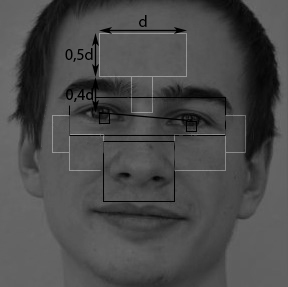
\includegraphics[width=8cm]{Obrazy/wyliczenieCzolka.jpg}
        \caption{Wyznaczenie strefy znajdującej się na czole.}
        \label{fig.wyznaczenieCzola}
    \end{figure}

    Autorzy~\cite{wrinkleFeatures} algorytmu założyli, że odległość od linii oczu do linii brwi wynosi $0,4 \cdot d$,
    natomiast wymiary ,,strefy czoła'' wynoszą $d \times 0,5d$.
    Na rysunku~\ref{fig.wspolrzedneDoWyliczeniaStref} przedstawiono współrzędne, które są pomocne w wyznaczaniu
    stref zmarszczkowych.

    \begin{figure}
        \centering
        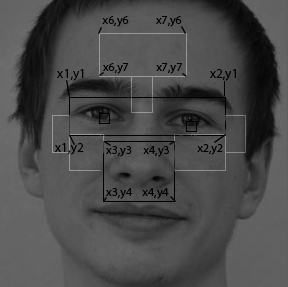
\includegraphics[width=9cm]{Obrazy/wspolrzedneDoWyliczeniaStref.jpg}
        \caption{Pomocnicze współrzędne do wyliczania stref zmarszczkowych.}
        \label{fig.wspolrzedneDoWyliczeniaStref}
    \end{figure}

    Strefa 2 została wyznaczona dzięki znajomości położenia prawego oka, dystansu między oczami oraz strefy ,,1''.
    Każda strefa może być wyznaczona przez jeden punkt (rysunek~\ref{fig.wykrywanieStrefZmarszczkowychPunkty})
    oraz jej wymiary.

    \begin{figure}
        \centering
        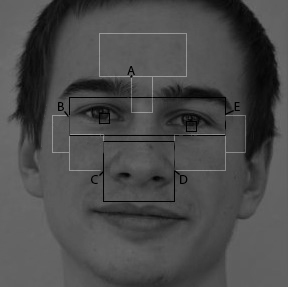
\includegraphics[width=8cm]{Obrazy/wykrywanieStrefZmarszczkowychPunkty.jpg}
        \caption{Punkty wyznaczające położenie stref.}
        \label{fig.wykrywanieStrefZmarszczkowychPunkty}
    \end{figure}

    Współrzędna x punktu A została wyznaczona ze wzoru~\ref{wzor.punktXA}

    \large
    \begin{equation}
        x_{A}=x_{6} + 0,375 \times d
        \label{wzor.punktXA}
    \end{equation}
    \normalsize
    gdzie $x_{6}$ to współrzędna z rysunku~\ref{fig.wspolrzedneDoWyliczeniaStref}.
    Natomiast $d$ jest odległością pomiędzy oczami (wzór~\ref{wzor.odlegloscPomiedzyOczami}).

    Współrzędną $y$ punktu A opisuje wzór~\ref{wzor.punktYA}:

    \large
    \begin{equation}
        y_{A}=y_{7}
        \label{wzor.punktYA}
    \end{equation}
    \normalsize
    Współrzędna $y_{7}$ analogicznie jak $x_{6}$ znajduje się na rysunku~\ref{fig.wspolrzedneDoWyliczeniaStref}.

    Zakładając, że prawe oko ma współrzędne $x_{o}$ oraz  $y_{o}$ wysokość strefy 2 wyznaczana jest w poniższy sposób
    (wzór~\ref{wzor.punktHA}).
    \large
    \begin{equation}
        h_{A}=y_{o}-y_{7}
        \label{wzor.punktHA}
    \end{equation}
    \normalsize

    Natomiast szerokość strefy 2 oblicza się następująco: (wzór~\ref{wzor.punktWA}):
    \large
    \begin{equation}
        w_{A}=0,25 \cdot d
        \label{wzor.punktWA}
    \end{equation}
    \normalsize
    Wartość 0,25 ze wzoru~\ref{wzor.punktWA} została dobrana empirycznie.

    Współrzędne punktu C (strefa 4) zostają wyznaczone ze wzoru~\ref{wzor.punktXC} oraz~\ref{wzor.punktYC}.
    \large
    \begin{equation}
        x_{C}=x_{3}
        \label{wzor.punktXC}
    \end{equation}
    \normalsize

    \large
    \begin{equation}
        y_{C}= \frac{y_{4} - y_{3}}{2}
        \label{wzor.punktYC}
    \end{equation}
    \normalsize

    Wysokość oraz szerokość strefy 4 (wzór~\ref{wzor.punktHC} oraz~\ref{wzor.punktWC})

    \large
    \begin{equation}
        h_{C}=y_{C} - y_{3}
        \label{wzor.punktHC}
    \end{equation}
    \normalsize

    \large
    \begin{equation}
        w_{C}= x_{3} - x_{1}
        \label{wzor.punktWC}
    \end{equation}
    \normalsize

    Strefa 5 zawiera punkt D - wzór~\ref{wzor.punktXD} oraz~\ref{wzor.punktYD}.

    \large
    \begin{equation}
        x_{D}=x_{4}
        \label{wzor.punktXD}
    \end{equation}
    \normalsize

    \large
    \begin{equation}
        y_{D}= y_{C}
        \label{wzor.punktYD}
    \end{equation}
    \normalsize

    Dla strefy 5 wyznacza się wysokość (wzór~\ref{wzor.punktHD}) oraz
    szerokość na podstawie wzoru (Wzór~\ref{wzor.punktWD}).

    \large
    \begin{equation}
        h_{D}=h_{C}
        \label{wzor.punktHD}
    \end{equation}
    \normalsize

    \large
    \begin{equation}
        w_{D}= x_{2} - x_{4}
        \label{wzor.punktWD}
    \end{equation}
    \normalsize

    Strefa 3 zawiera punkt B wyznaczany ze wzorów~\ref{wzor.punktXB} i~\ref{wzor.punktYB}

    \large
    \begin{equation}
        x_{B}=x_{1}
        \label{wzor.punktXB}
    \end{equation}
    \normalsize

    \large
    \begin{equation}
        y_{B}= \frac{y_{2} - y_{1}}{2}
        \label{wzor.punktYB}
    \end{equation}
    \normalsize

    Wysokość (wzór~\ref{wzor.punktHB}) oraz szerokość (wzór~\ref{wzor.punktWB}) strefy 3.

    \large
    \begin{equation}
        h_{B}=y_{C} - y_{B}
        \label{wzor.punktHB}
    \end{equation}
    \normalsize

    \large
    \begin{equation}
        w_{B}= w_{C} * 0,4
        \label{wzor.punktWB}
    \end{equation}
    \normalsize

    Na samym końcu zostaje wyznaczona strefa 6.
    Wyznaczona zostaje współrzędna E - wzór~\ref{wzor.punktXE} i~\ref{wzor.punktYE}.
    \large
    \begin{equation}
        x_{E}=x_{2}
        \label{wzor.punktXE}
    \end{equation}
    \normalsize

    \large
    \begin{equation}
        y_{E}= y_{B}
        \label{wzor.punktYE}
    \end{equation}
    \normalsize

    Szerokość oraz wysokość strefy 6.

    \large
    \begin{equation}
        h_{E}=h_{B}
        \label{wzor.punktHE}
    \end{equation}
    \normalsize

    \large
    \begin{equation}
        w_{E}= w_{D} \cdot 0,4
        \label{wzor.punktWE}
    \end{equation}
    \normalsize

    Należy zauważyć, że szerokość stref 3 i 6 jest pomnożona przez 0,4 szerokości odpowiednio
    stref 4 i 5.
    Wartość ,,0,4'' została dobrana empirycznie.
    \section{Wykrywanie zmarszczek - detektor Canny}\label{sec:wykrywanie-zmarszczek---detektor-canny}
    %opis detektora z wiki angielskiej
    Następnym krokiem algorytmu po wyznaczeniu stref zmarszczkowych jest wyodrębnienie zmarszczek poprzez detekcję
    krawędzi.
    Istnieje wiele metod do tego celu,
    jednak detektor Canny jest jedną z najbardziej dokładnych i niezawodnych, dlatego został zastosowany w toku badań.
    Metoda ta została opracowana przez Johna F. Canny w 1986 roku.
    Oprócz samej implementacji algorytmu jego twórca zaprezentował teorię obliczeniową,
    która wyjaśnia działanie tej metody. Ponadto Canny zauważył,
    że wymagania dotyczące implementacji detekcji krawędzi są podobne do siebie w wielu systemach wizyjnych.
    W związku z powyższym jego algorytm może zostać skutecznie zastosowany w różnych systemach tego typu.
    Poniżej przedstawiono najważniejsze zasady,
    które są niezbędne do dobrej detekcji krawędzi w opisywanym algorytmie:
    \begin{itemize}
        \item Detekcja krawędzi z niskim prawdopodobieństwem błędu:
        Oznacza to, że algorytm powinien wykryć jak najwięcej krawędzi, które rzeczywiście istnieją.
        Natomiast ilość krawędzi wykrytych błędnie powinna być jak najmniejsza.
        \item Precyzja detekcji: Algorytm powinien precyzyjnie zlokalizować krawędź dokładnie w jej środku.
        \item Brak redundantnych detekcji:
        Krawędź powinna być zlokalizowana jednokrotnie,
        a szum na obrazie nie powinien generować dodatkowych krawędzi.
    \end{itemize}
    W algorytmie detekcji Canny używa rachunku wariacyjnego.
    Rachunek wariacyjny to dziedzina analizy matematycznej, która
    analizuje przestrzenie funkcyjne i znajduje w nich ekstrema funkcjonałów.
    Funkcjonały natomiast przekształcają przestrzeń wektorową na liczby rzeczywiste.
    Zatem rachunek wariacyjny ma za zadanie pomóc w znalezieniu charakterystycznej funkcji,
    dla której funkcjonał przyjmuje wartość ekstremalną.
    Algorytm detektora jest podzielony na kilka kroków~\cite{Canny}:
    \begin{itemize}
        \item Redukcja szumów na obrazie filtrem Gaussa.
        \item Szukanie gradientów jasności.
        \item Zastosowanie techniki zmniejszania grubości krawędzi.
        \item Likwidacja krawędzi o małym gradiencie jasności.
        \item Filtracja poprzez histerezę.
    \end{itemize}
    \subsection*{Redukcja szumów na obrazie filtrem Gaussa}\label{subsec:redukcja-szumów-na-obrazie-filtrem-gaussa}
    Szum na obrazie to piksele o losowym kolorze, jasności oraz umiejscowieniu (współrzędnych na obrazie).
    Takie piksele są nadmiarowymi informacjami o obrazie oraz stanowią efekt uboczny przetwarzania obrazu
    przez matrycę cyfrową (rysunek~\ref{fig.lenkaSzumy}).

    \begin{figure}[h!]
        \centering
        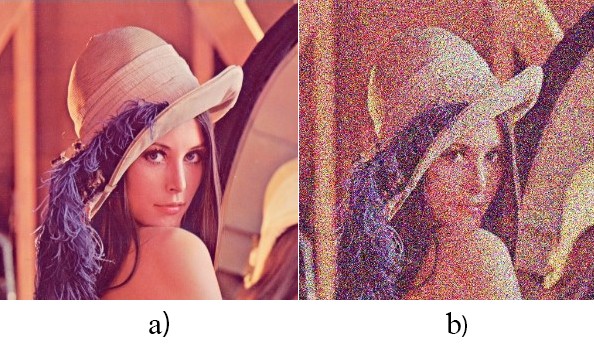
\includegraphics[width=11cm]{Obrazy/lenkaSzumy.jpg}
        \caption{a) Obraz z nieznaczną ilością szumów b) Obraz ze znaczną ilością szumów~\cite{lenkaSzumy}.}
        \label{fig.lenkaSzumy}
    \end{figure}

    Efekt szumu jest spotykany również w fotografii analogowej.
    W fotografii cyfrowej szum wzrasta na skutek zwiększania czułości matrycy lub przez wzrost jej temperatury.
    Redukcję szumów można uzyskać stosując filtr Gaussa.
    Splot filtru Gaussa z obrazem daje w wyniku wygładzony obraz ze zmniejszoną ilością szumów.
    Filtr Gaussa może mieć różne wymiary.
    Rozmiar filtra ma wpływ na wydajność wygładzania obrazu, a co za tym idzie na czułość wykrywania szumu~\cite{Canny}.
    \subsection*{Szukanie gradientów jasności}\label{subsec:szukanie-gradientów-jasności}
    Istotnym parametrem w wykrywaniu krawędzi jest gradient jasności.
    Określa on jak bardzo zmienia się jasność danego piksela względem sąsiadujących pikseli.
    Gradient jasności otrzymany zostaje ze wzoru~\ref{wzor.gradientJasnosci}:
    \large
    \begin{equation}
        G = \sqrt{G_{x}^{2} + G_{y}^{2}}
        \label{wzor.gradientJasnosci}
    \end{equation}
    \normalsize
    gdzie $G_{x}$ jest zmianą jasności danego piksela w kierunku poziomym, a $G_{y}$ w kierunku pionowym.
    Kierunek gradientu opisuje wzór~\ref{wzor.kierunekGradientu}
    \large
    \begin{equation}
        \Theta = atan2(G_{y}, G_{x})
        \label{wzor.kierunekGradientu}
    \end{equation}
    \normalsize
    Krawędzie na obrazie charakteryzują się pewną zmianą jasności na danym obszarze obrazu.
    Krawędź na obrazie może być położona pod różnym kątem.
    Opisywany detektor używa czterech filtrów w celu wykrycia pionowych, poziomych oraz ukośnych krawędzi.

    Kierunek gradientu jest zaokrąglony do jednego z filtrów kierunku: poziomego ($\Theta = 0^{\circ}$),
    pionowego ($\Theta = 90^{\circ}$) lub ukośnego ($\Theta = 45^{\circ}$
    lub $\Theta = 135^{\circ}$ stopni).
    Każdy piksel obrazu otrzymuje wartość gradientu (wzór~\ref{wzor.gradientJasnosci})
    oraz kierunek - zgodny z powyższym filtrem kierunku.
    W wyniku tego działania otrzymuje się obraz gradientowy~\cite{Canny}.
    \subsection*{Zastosowanie techniki zmniejszania grubości
    krawędzi}\label{subsec:zastosowanie-zmniejszania-grubości-krawędzi}
    Zmniejszanie grubości krawędzi służy do filtracji krawędzi powstałych po poprzednim kroku.
    Krawędzie wykryte za pomocą gradientu są rozmyte.
    Dzięki technice zmniejszania grubości można odszukać na małym obszarze gradienty o największej wartości
    , które identyfikują najostrzejsze krawędzie.
    Wszystkie inne, o mniejszej wartości, są ignorowane.
    Algorytm operuje na obrazie gradientowym powstałym jako wynik działania algorytmu opisanego w sekcji~\ref{subsec:szukanie-gradientów-jasności}
    Działa on następująco:

    Odczytana zostaje wartość gradientu oraz jego kierunek dla danego piksela.
    Następnie wartość gradientu porównuje się z wartościami gradientu dla
    dwóch sąsiednich pikseli.
    Sąsiednie piksele leżą na jednej linii wyznaczonej przez kierunek gradientu.
    Jeśli wartość danego piksela jest największa spośród pikseli wzdłuż wyżej wymienionych linii,
    to dany piksel należy do najostrzejszej krawędzi~\cite{Canny}.

    \subsection*{Filtracja krawędzi o małym gradiencie
    jasności}\label{subsec:filtracja-krawędzi-o-małym-gradiencie-jasności}
    Zastosowanie techniki zmniejszania grubości krawędzi pozostawia na obrazie wiele krawędzi, które są wygenerowane przez szum i zmiany
    kolorów.
    Kolejnym krokiem jest filtracja powyższych krawędzi, gdyż są one nadmiarowe.
    W tym celu ustawiany jest pewien próg, zwany progiem małym $T_{l}$.
    Oprócz progu małego ustawiany jest również próg duży $T_{h}$ w celu wyodrębnienia krawędzi o wysokim gradiencie
    jasności.
    Jeśli wartość gradientu dla danej krawędzi jest mniejsza od progu małego, to zostaje ona usunięta.
    W przypadku, gdy wartość jest większa od progu małego, ale mniejsza od progu dużego, dana krawędź
    zostaje oznaczona jako słaba.
    Krawędź oznacza się jako mocną, gdy wartość gradientu dla niej jest większa od wartości progu dużego~\cite{Canny}.

    \subsection*{Filtracja poprzez histerezę}\label{subsec:filtracja-poprzez-histerezę}
    W wyniku działania algorytmu do tej pory zostały uzyskane słabe oraz mocne krawędzie.
    Mocne krawędzie zostaną oznaczone jako prawdziwe krawędzie znajdujące się na obrazie.
    Słabe krawędzie mogą być częścią mocnych krawędzi, ale
    mogą również zostać wygenerowane przez szum lub zmiany kolorów.
    Krawędzie tego typu nie są prawdziwymi krawędziami w obrazie, więc w ostatnim kroku algorytmu powinny zostać
    przefiltrowane.
    Słabe krawędzie, które są powiązane z mocnymi znajdują się w najbliższym sąsiedztwie mocnych krawędzi.
    W celu odnalezienia tych powiązań pomiędzy krawędziami zostaje zastosowana analiza spójności krawędzi.
    Jeśli zostaje zidentyfikowane powiązanie pomiędzy mocną, a słabą krawędzią, to słabą krawędź pozostawia się w obrazie.
    W przypadku, gdy słaba krawędź nie jest powiązana z żadną mocną krawędzią - zostaje usunięta~\cite{Canny}.

    \section{Wyliczanie współczynnika zmarszczek}\label{sec:wyliczanieWrinkleFeature}
    W wyniku działania detektora Cannego, który został opisany w sekcji~\ref{sec:wykrywanie-zmarszczek---detektor-canny}
    wygenerowany zostaje obraz binarny z wyodrębnionymi krawędziami.
    Obraz binarny zawiera piksele o dwóch wartościach jasności pikseli.
    Piksel może być albo biały albo czarny.
    Krawędzie można rozpoznać jako białe piksele, natomiast czarne piksele oznaczają brak krawędzi (rysunek~\ref{fig.mojaTwarzGray}).

    \begin{figure}[h!]
        \centering
        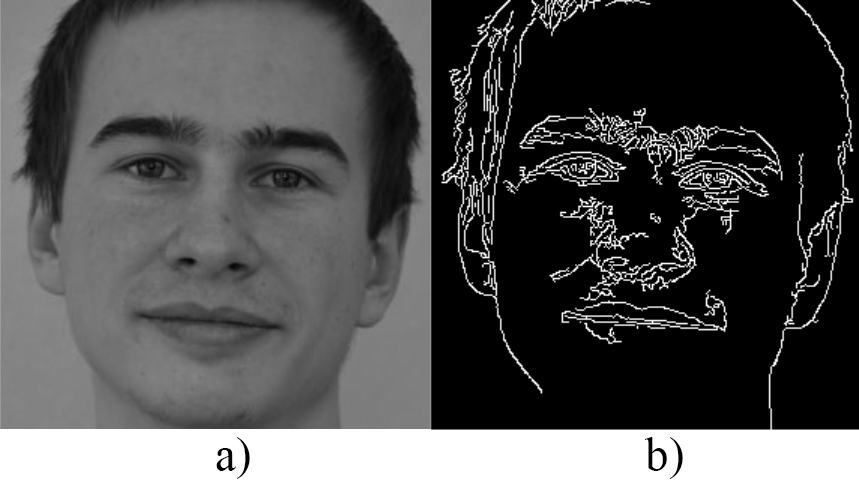
\includegraphics[width=11cm]{Obrazy/mojaTwarzGray.jpg}
        \caption{a) Oryginalny obraz b) Obraz z wykrytymi krawędziami.} %todo musi byc nizej
        \label{fig.mojaTwarzGray}
    \end{figure}

    Na rysunku~\ref{fig.mojaTwarzGray} widoczne są krawędzie, które identyfikują owal twarzy.
    Ponadto widoczne są poszczególne części twarzy tj. nos, oczy, brwi.
    Można także zauważyć dodatkowe krawędzie w strefach zmarszczkowych (sekcja~\ref{sec:wyznaczanieStref}),
    które identyfikują zmarszczki.
    W metodzie bazowej ilość białych pikseli w strefach zmarszczkowych jest wprost proporcjonalna do ilości zmarszczek
    na twarzy danej osoby.

    Z każdej strefy zmarszczkowej obliczany jest stosunek ilości białych pikseli do wszystkich
    pikseli (wzór~\ref{wzor.wspolczynnikZmarszczek}).
    \large
    \begin{equation}
        W_{s1} = \frac{PB_{s1}}{PW_{s1}}
        \label{wzor.wspolczynnikZmarszczek}
    \end{equation}
    \normalsize
    gdzie $W_{s1}$ jest stosunkiem białych pikseli do wszystkich w strefie 1,
    $PB_{s1}$ - suma białych pikseli w strefie 1, $PW_{s1}$ - suma wszystkich pikseli w strefie 1.
    Analogicznie obliczane są stosunki pikseli dla pozostałych stref.
    Ostatnim etapem jest sumowanie wszystkich stosunków pikseli (wzór~\ref{wzor.wrinkleFeature}).
    \large
    \begin{equation}
        WZ = W_{s1} + W_{s2} + W_{s3} + W_{s4} + W_{s5} + W_{s6}
        \label{wzor.wrinkleFeature}
    \end{equation}
    \normalsize
    gdzie WZ to wskaźnik zmarszczek - parametr określający ilość zmarszczek dla danej osoby.

    \section{Algorytm analizy danych ze zbioru trenującego}\label{sec:algorytmTrenowania}
    W celu skonstruowania programu wyznaczającego wiek na podstawie tekstury należy wcześniej zbadać zależność ilości
    zmarszczek od wieku.
    W tym celu należy posiadać odpowiednią bazę zdjęć, na których można przeprowadzić wyżej wspomniane badania.

    Jest wiele darmowych źródeł obrazów twarzy.
    Najczęściej używane bazy to FG-NET oraz MORTH II, które
    zawierają dziesiątki tysięcy zdjęć.
    Zdjęcia są różnej jakości i nie każda baza zdjęć nadaje się do konkretnych badań~\cite{khryashchevGanin}.
    Przy realizacji tej pracy wykorzystana została baza UTKFace,
    ponieważ wszystkie zgrupowane w niej obrazy przedstawiają twarze w pozycji frontalnej. Dodatkowo
    ścieżka pliku każdego obrazu zawiera informacje na temat rzeczywistego wieku, co pozwala w łatwy sposób
    zweryfikować poprawność algorytmu.
    W związku z powyższym z każdego zdjęcia z tej bazy otrzymywano dwie informacje - rzeczywisty wiek danej osoby oraz
    współczynnik zmarszczek.
    Następnie dla całej bazy wygenerowano zbiór danych, który w dalszej kolejności był odpowiednio analizowany w celu
    sprawdzenia zależności pomiędzy współczynnikiem zmarszczek, a wiekiem.
    Autorzy algorytmu w celu analizy uprzednio wygenerowanego zbioru danych wykorzystali algorytm grupowania -
    Fuzzy C-Means.
    W wyniku działania tego algorytmu otrzymuje się informacje, dzięki którym na podstawie współczynnika zmarszczek
    można
    oszacować wiek~\cite{wrinkleFeatures}.
    \section{Grupowanie danych - Fuzzy C-Means oraz wyznaczanie wieku}\label{sec:grupowanieDanych}
    %    https://pl.wikipedia.org/wiki/Analiza_skupień
    %    https://en.wikipedia.org/wiki/Cluster_analysis
    %    https://sci-hub.tw/10.1109/ICCSA.2019.000-1
    %    https://www.researchgate.net/publication/329424581_Data_clustering
    %    Podac rozne przyklady algorytmow - hierarchiczne, niehierarchiczne
    %mozna dopisac o roznych odleglosciach stosowanych do przydzielania do klastrow
    Grupowanie danych, zwane również klasteryzacją, jest szeroko stosowane w uczeniu maszynowym, rozpoznawaniu wzorców,
    analizie obrazu, bioinformatyce, kompresji danych czy w grafice komputerowej.
    Polega na podzieleniu dużego zbioru danych na grupy.
    Powyższe grupy zawierają dane, które są podobne do siebie~\cite{clusterWstep}.

    Klasteryzacja jest zadaniem, które może zostać wykonane na wiele sposobów.
    Jest również iteracyjnym procesem odkrywania danych w celu odnalezieniu relacji pomiędzy nimi.

    Odpowiedni algorytm grupowania i ustawienia parametrów (w tym parametrów
    takich jak funkcja odległości lub liczba oczekiwanych grup)
    zależą od zestawu danych i sposobu wykorzystania wyników.
    Dane nieraz muszą zostać przefiltrowane lub potrzebna jest zmiana parametrów grupowania w celu osiągnięcia
    zamierzonego efektu~\cite{clusterWstep}.

    Najczęściej grupa jest definiowana przez jak najmniejszą odległość pomiędzy jej członkami.
    Zarazem odległość pomiędzy członkami grupy jest głównym parametrem klasteryzacji hierarchicznej.
    Istnieje również wiele innych modeli grupowania.
    Jednym z nich jest model centroidowy,
    który zakłada, że każda grupa jest zdefiniowana przez jeden wektor, posiadający wartość średnią.
    Istnieją też modele, które opierają się na sieciach neuronowych.
    Ich podstawą jest założenie, że dane grupują się za pomocą nienadzorowanych sieci neuronowych.
    Spotykany jest także model oparty o rozkłady statystyczne.

    Klasteryzacja może być twarda lub miękka.
    Twarda klasteryzacja oznacza, że każdy element danych może należeć tylko do jednej grupy.
    Natomiast w przypadku miękkiej klasteryzacji każdy element danych może w pewnym stopniu należeć do każdej z grup.
    Autorzy algorytmu szacowania wieku będącego podstawą przeprowadzonych badań zastosowali grupowanie metodą Fuzzy
    C-means.
    Należy ona do grupy modeli centroidowych~\cite{clusterWstep}. W Fuzzy C-means zastosowano klasteryzacje miękką.

    %- dokladny opis jak to dziala
    %    https://sci-hub.tw/10.1007/s12046-019-1166-1
    %pozniej opisac co otrzymalismy w wyniku dzialania algorytmu, ze tam byly centroidy wraz z wartoscia
    Algorytm Fuzzy C-means został stworzony w 1973 przez J. C. Dunn. Po raz pierwszy został opisany w
    książce~\cite{ISODATA}.

    Klasteryzacja Fuzzy C-means dzieli zbiór $S$ na podzbiory $s_{i}$ zgodnie ze wzorem~\ref{wzor.zbiorX}):
    \large
    \begin{equation}
        S:=\{s_{1},s_{2},s_{3},\ldots,s_{N}\}\subset \mathbb{R}
        \label{wzor.zbiorX}
    \end{equation}
    \normalsize
    W parametrze algorytmu zostaje ustalona liczba grup $N$.
    Każda grupa posiada charakterystyczną wartość nazywaną centroidem $p_{j}\subset \mathbb{R}$.
    Jak zostało wspomniane na początku tego rozdziału, w algorytmie C-means zastosowana jest miękka klasteryzacja.
    Każdy element danych $x_{i}$ ma przypisywany wektor $U_{i}$ przynależności do grupy
    (wzór~\ref{wzor.wektorPrzynaleznosci}).
    \large
    \begin{equation}
        U_{i}=(u_{i1}, u_{i2}, u_{i3}, \ldots, u_{ic})
        \label{wzor.wektorPrzynaleznosci}
    \end{equation}
    \normalsize
    gdzie $u_{i1}$ oznacza stopień przynależności elementu $x_{i}$ do grupy 1.
    Analogicznie $u_{i2}$ oznacza stopień przynależności elementu $x_{i}$ do grupy 2.

    W pierwszym kroku zbiór centroidów P jest inicjalizowany losowo (wzór~\ref{wzor.zbiorCentroidow}).
    \large
    \begin{equation}
        P^{0}=(p_{1}^{0}, p_{2}^{0}, p_{3}^{0}, \ldots, p_{c}^{0})
        \label{wzor.zbiorCentroidow}
    \end{equation}
    \normalsize
    W k-tym kroku algorytmu wyliczona jest macierz funkcji przynależności $U^{k} = {u_{ij}^{k}}$ (wzór~\ref{wzor.funkcjaPrzynaleznosci}).
    \large
    \begin{equation}
        u_{ij}^{k} = \frac{1}{\sum_{k=1}^{c}\left ( \frac{\left \| x_{i} - p_{j}^{k} \right \|}{\left \|x_{i} - p_{k}^{k}  \right \|} \right )^{\frac{2}{m-1}}}
        \label{wzor.funkcjaPrzynaleznosci}
    \end{equation}
    \normalsize
    Wyrażenie $\left \| x_{i} - p_{j} \right \|$ oznacza odległość Euklidesową pomiędzy elementem $x_{i}$ a
    centroidem $p_{j}$. Parametr ,,m'' jest nazywany współczynnikiem rozmycia. Współczynnik ten może być w zakresie
    od 1 do nieskończoności, jednak w większości przypadków jest równy 2.

    W kroku $(k+1)^{th}$ centroid $p_{j}^{(k+1)}$ jest uaktualniany według wzoru~\ref{wzor.kaPLusJeden}.
    \large
    \begin{equation}
        p_{j}^{(k+1)}=\frac{\sum_{i=1}^{n}u_{ij}^{(k+1)m}x_{j}}{\sum_{i=1}^{n}u_{ij}^{(k+1)m}}
        \label{wzor.kaPLusJeden}
    \end{equation}
    \normalsize
    Algorytm w kolejnych iteracjach minimalizuje funkcję przynależności $J(U,P)$ podaną wzorem~\ref{wzor.kryteriumFCM}:

    \large
    \begin{equation}
        J(U,P)= \sum_{i=1}^{n}\sum_{j=1}^{c}u_{ij}^{m}\left \| x_{i}-p_{j} \right \|^{2}
        \label{wzor.kryteriumFCM}
    \end{equation}
    \normalsize
    Iteracje kończą się, gdy zostanie osiągnięty warunek opisany wzorem~\ref{wzor.koniecIteracjiWarunek}
    \large
    \begin{equation}
        \left \| J^{(k+1)}(U,P) - J^{(k)}(U,P)) \right \| < \epsilon
        \label{wzor.koniecIteracjiWarunek}
    \end{equation}
    \normalsize
    gdzie $\epsilon > 0$. Parametr $\epsilon$ jest parametrem ustawianym przed uruchomieniem klasteryzacji.
    W niektórych implementacjach istnieje możliwość zakończenia działania algorytmu po określonej liczbę iteracji,
    jeśli wcześniej nie zostanie osiągnięte kryterium ze wzoru~\ref{wzor.koniecIteracjiWarunek}.

    Po zakończeniu działania wyżej opisanego algorytmu zostaje wyliczony wektor przynależności $U$
    (wzór~\ref{wzor.wektorPrzynaleznosci}). Wektor ten opisuje stopień przynależności elementu $f_{i}$ do
    poszczególnych klastrów.
    %    U_{i}=(u_{i1}, u_{i2}, u_{i3}, \ldots, u_{ic})
    Suma wektora przynależności $U_{i}$, dla elementu $x_{i}$ jest opisana
    wzorem~\ref{wzor.sumaWektorPrzynaleznosci}
    \large
    \begin{equation}
        \sum_{j=0}^{j=c} u_{ij}=1
        \label{wzor.sumaWektorPrzynaleznosci}
    \end{equation}
    \normalsize
    gdzie c oznacza liczbę klastrów.
    Element $f_{i}$ będzie należał do klastra k, jeśli $u_{ik}$ ma największą wartość w wektorze $U_{i}$.

    W tym akapicie zostanie przedstawiony algorytm trenowania za pomocą Fuzzy C-means.
    Z każdego zdjęcia ,,i'' otrzymywane są dane dotyczące rzeczywistego wieku $A_{i}$ oraz parametr wskaźnika
    zmarszczek
    $WF_{i}$.
    W algorytmie Fuzzy C-means są grupowane zbiory danych zawierające wartości wskaźnika zmarszczek $WF_{i}$.
    Jak wiadomo z powyższego opisu algorytmu Fuzzy C-means, każdy element (w tym przypadku $WF_{i}$) ma określony
    stopień
    przynależności do każdego klastra. Dany element $WF_{i}$ będzie należał do klastra o największym stopniu
    przynależności. Każde zdjęcie jest grupowane według wyżej opisanego algorytmu FCM.

    Każdy klaster ma określony centroid j, który posiada parametr $P_{wfj}$  oraz dodatkowy parametr - średnią
    wartość wieku $P_{aj}$. $P_{wfj}$ oznacza wartość wskaźnika zmarszczek dla danego centroida.
    $P_{aj}$ jest wyznaczany ze wzoru~\ref{wzor.avgJ}.
    \large
    \begin{equation}
        P_{aj}=\frac{\sum_{}^{}A_{i}}{N_{j}}
        \label{wzor.avgJ}
    \end{equation}
    \normalsize
    gdzie $A_{i}$ to rzeczywisty wiek osoby z obrazu $i$, który należy do klastru $j$.
    Natomiast $N_{j}$ to liczba zdjęć zaklasyfikowanych do klastru $j$.

    W powyższym akapicie został opisany algorytm klasteryzacji, który generuje $N$ centroidów, reprezentujących każdą
    grupę. Natomiast osobnym etapem jest szacowanie wieku.
    W pierwszej fazie działanie algorytmu jest dokładnie takie same jak w sekcjach od~\ref{sec:metodaWykrywaniaTwarzy}
    do~\ref{sec:wyliczanieWrinkleFeature}:
    Algorytm szacowania wieku w pierwszej kolejności dokonuje detekcji twarzy, oczu, ust na danym obrazie $O_{i}$.
    Jeśli powyższe elementy zostały zidentyfikowane, wyznaczane są strefy zmarszczkowe,
    a następnie zostaje wyliczony parametr wskaźnik zmarszczek $WF_{i}$~\cite{wrinkleFeatures}.

    %    Należy podkreślić, że zdjęcia do testowania algorytmu szacowania wieku
    %    pochodzą z innej bazy obrazów niż obrazy wykorzystane w treningu. Ma to na celu eliminację błędów w testowaniu algorytmu.
    %    Każdy centroid posiada parametr
    %    W wyniku działania algorytmu wygenerowanych zostaje n grup. Każda grupa posiada centroid wraz ze średnim wiekiem.


    Dla parametru $WF_{i}$ zostaje wyznaczony wektor przynależności do grupy
    według wzoru~\ref{wzor.wektorPrzynaleznosci}.
    Przy założeniu dla wektoru przynależności zgodnym ze wzorem~\ref{wzor.sumaWektorPrzynaleznosci} szacowany wiek
    $PA$
    wynosi
    (wzór~\ref{wzor.szacowanyWiek}).
    \large
    \begin{equation}
        PA=\sum_{j=1}^{N}(u_{ij} \cdot P_{aj})
        \label{wzor.szacowanyWiek}
    \end{equation}
    \normalsize
    gdzie $u_{ij}$ oznacza przynależność i-tego zdjęcia do j-tego klastra, $N$ oznacza liczbę klastrów, podaną jako
    parametr wejściowy algorytmu FCM,
    natomiast $P_{aj}$ jest średnim wiekiem dla j-tego centroida.
    %    Zbiór zdjęć użytych do treningu wynosi około 22000.
    % opisac wraz z przykladem moze jakis rysuneczek.

    %Tutaj powinno byc 5000 slow
    \chapter{Modyfikacje metody bazowej}\label{ch:modyfikacje-metody-bazowej}
    W sekcji~\ref{sec:odjęcie-wybranej-strefy} zostanie przedstawiona pierwsza modyfikacja algorytmu bazowego.
    Kolejna sekcja~\ref{sec:zastosowanie-metody-hog} zawiera opis kolejnej modyfikacji algorytmu, w której użyto
    algorytm HOG-a.
    W ostatniej sekcji~\ref{sec:metoda-hog-oraz-algorytm-knn} została zaprezentowana ostatnia modyfikacja, która oprócz algorytmu HOG do szacowania
    wieku wykorzystuje algorytm KNN.

    \section{Odjęcie wybranej strefy}\label{sec:odjęcie-wybranej-strefy}
    Pierwsza modyfikacja polegała na odjęciu jednej wybranej strefy. Detektor Canny oprócz zmarszczek
    wykrywa także włosy. Podczas przeglądania wielu zdjęć zauważono, że w obrębie
    strefy zmarszczek nr 2 (obraz~\ref{fig.wykrywanieStrefZmarszczkowych}) wykrywane są części brwi oprócz samych
    zmarszczek. Generuje to błąd, dlatego wyżej wymienionej strefy nie uwzględniono w obliczeniach.
    W sekcji~\ref{subsec:zmiana-algorytmu-względem-metody-bazowej} porównano różnice w algorytmie przed opisaną wyżej
    modyfikacją i po niej.

    \subsection*{Zmiana algorytmu względem metody bazowej}\label{subsec:zmiana-algorytmu-względem-metody-bazowej}
    Przed modyfikacją metody bazowej parametr wskaźnika zmarszczek był obliczany według wzoru~\ref{wzor.wrinkleFeature},
    który jest umieszczony w sekcji~\ref{sec:wyliczanieWrinkleFeature}.

    Po modyfikacji wskaźnik zmarszczek oblicza się według wzoru~\ref{wzor.wrinkleFeature2}.
    \large
    \begin{equation}
        WZ = W_{s1} + W_{s3} + W_{s4} + W_{s5} + W_{s6}
        \label{wzor.wrinkleFeature2}
    \end{equation}
    \normalsize
    Kolejną modyfikacją było zastosowanie metody HOG (ang. Histogram of Oriented Gradients), która została opisana w
    sekcji~\ref{sec:zastosowanie-metody-hog}.

    \section{Opis metody HOG}\label{sec:zastosowanie-metody-hog}
    %https://sci-hub.tw/10.2139/ssrn.3268935
    %https://www.learnopencv.com/histogram-of-oriented-gradients/
    %    https://en.wikipedia.org/wiki/Histogram_of_oriented_gradients
    %    https://hal.inria.fr/inria-00548512/document
    Metoda HOG jest deskryptorem cech z obrazu.
    Deskryptor cech wyodrębnia z obrazu pewne cechy, do których należą między innymi kolory czy tekstury.
    W metodzie bazowej rolę deskryptora tego rodzaju spełnia detektor
    krawędzi Canny (sekcja~\ref{sec:wykrywanie-zmarszczek---detektor-canny}), który wykrywa krawędzie,
    identyfikowane jako zmarszczki.
    Z kolei Histogram of Oriented Gradients jest techniką, która liczy wystąpienia kierunków gradientów jasności.
    Metoda HOG została zaimplementowana w 2005 roku przez Navneeta Dalala i Billa
    Triggsa~\cite{hogZabojady}.
    Została wtedy zastosowana do detekcji pieszych na zdjęciach.
    Później jej zastosowanie rozszerzono o wykrywanie ludzi w filmach wideo,
    ponadto stosowano ją także do wykrywania zwierząt oraz pojazdów na zdjęciach.

    Metoda Histogram of Oriented Gradients opiera się na założeniu, że wygląd i kształt obiektów na obrazie może zostać
    opisany przez gradient jasności oraz jego kierunek. Jest to dobrze widoczne na
    rysunku~\ref{fig.gradientJasnosciNaGlowie}

    \begin{figure}
        \centering
        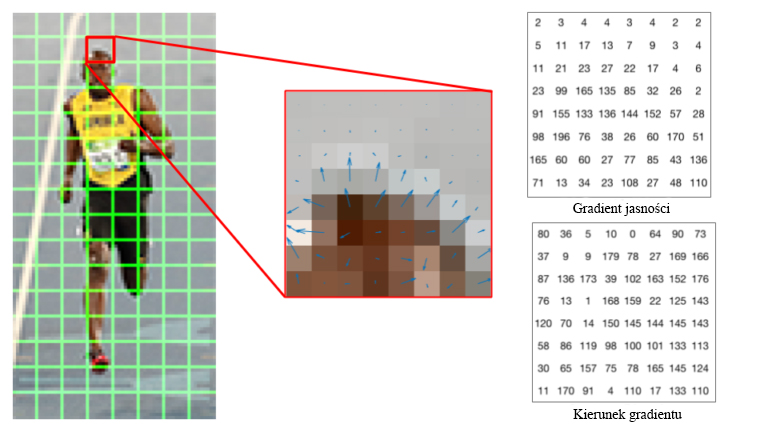
\includegraphics[width=11cm]{Obrazy/gradientJasnosciNaGlowie.jpg}
        \caption{Gradient jasności identyfikujący granicę pomiędzy głową a tłem~\cite{hogOpenCv}.}
        \label{fig.gradientJasnosciNaGlowie}
    \end{figure}
    Na granicy pomiędzy tłem, a głową sportowca widoczne są duże wartości gradientu jasności.
    W ten sposób zostaje zidentyfikowana krawędź głowy.

    Działanie algorytmu można pokrótce opisać w następujący sposób. Obraz jest dzielony na małe obszary zwane komórkami,
    które zwykle mają wymiar kilka na kilka pikseli. Komórki są grupowane w bloki, mogące składać się z różnej ilości
    komórek.
    Dla wszystkich pikseli w komórce tworzony jest histogram kierunków gradientu.
    Następnie histogramy są łączone w jeden wspólny deskryptor.
    Dla zwiększenia dokładności lokalne histogramy normalizowane są pod względem kontrastu.
    Realizowane jest to przez pomiar jasności w bloku. Normalizacja zapewnia zmniejszenia niepożądanego efektu
    generowanego przez
    różnice w oświetleniu różnych obszarów zdjęcia. Wspomniana sytuacja występuje na przykład, gdy zdjęcie wykonywane
    jest w nieprawidłowych warunkach oświetleniowych (rysunek~\ref{fig.oswietlenieTwarzy}).

    W pierwszej fazie algorytmu HOG obraz powinien zostać przeskalowany, tak aby jego wymiary były podzielne przez
    rozmiar
    pojedynczej komórki.
    (rysunek~\ref{fig.komorkiHoga}).
    \begin{figure}
        \centering
        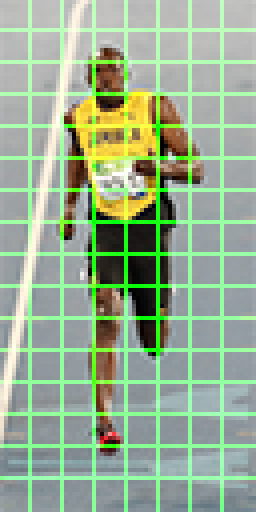
\includegraphics[width=4cm]{Obrazy/komorkiHoga.jpg}
        \caption{Komórki o rozmiarze 8x8 pikseli na zdjęciu~\cite{hogOpenCv}.}
        \label{fig.komorkiHoga}
    \end{figure}
    Warto wspomnieć, że w wielu metodach generujących deskryptory pierwszą fazą jest korekcja luminancji.
    Jednak ten krok może zostać pominięty, gdyż w późniejszym kroku stosowana jest normalizacja,
    która dokonuje korekcji luminancji cieni oraz świateł.
    W kolejnej fazie muszą zostać wyznaczone gradienty jasności.
    Wyznaczenie gradientów jasności zostało szczegółowo opisane w sekcji~\ref{subsec:szukanie-gradientów-jasności}.
    W kolejnej fazie zostają wyznaczone histogramy gradientów dla każdej komórki.
    Na rysunku~\ref{fig.gradientJasnosciNaGlowie} został przedstawiony wynik działania tego kroku.
    Zostają wygenerowane dwie macierze. Pierwsza zawiera informację o gradiencie jasności każdego piksela komórki,
    natomiast druga - informację o kierunku każdego gradientu.
    Wartości kierunku gradientu wyrażone są w stopniach. W metodzie Histogram of Oriented Gradients
    zastosowano kierunki gradientu bez znaku. Oznacza to, że zakres kierunków mieści się w granicach
    od $0^{\circ}$ do $180^{\circ}$.
    Użycie kierunku gradientu bez znaku jest uzasadnione tym,
    że wartość kierunku o takiej samej wartości, lecz różnych znakach reprezentuje gradient o tym samym kierunku, lecz
    różnych zwrotach. Dla detekcji kształtów krawędzi czy kształtów istotny jest kierunek, a nie zwrot.
    Na podstawie kierunku gradientu oraz wartości gradientu jasności zostaje wygenerowany histogram gradientów.
    W parametrze wejściowym algorytmu HOG ustawiana jest ilość kubełków histogramu.
    Najczęściej stosuje się 9 kubełków. Każdy kubełek histogramu odpowiada pewnemu zakresowi kąta kierunku gradientu.
    Przykładowo dla histogramu o szerokości 9 kubełków każdy kubełek odpowiada przedziałom $20^{\circ}$ wycentrowanym
    dla podanych wartości:
    $0^{\circ}$, $20^{\circ}$, $40^{\circ}$, \ldots, $160^{\circ}$.
    Na rysunku~\ref{fig.hogTworzenieHistogramu} przedstawiono sposób przypisywania wartości do kubełków histogramu.
    \begin{figure}
        \centering
        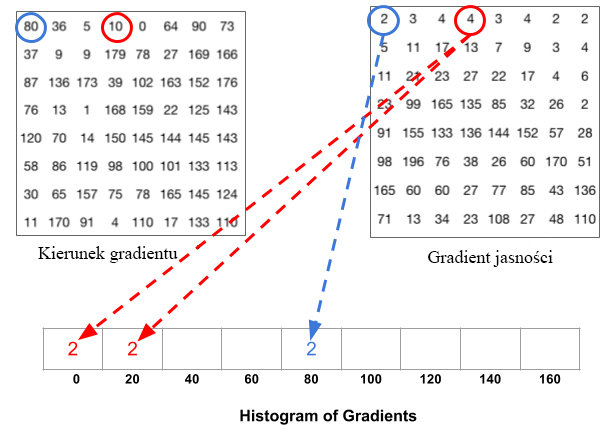
\includegraphics[width=11cm]{Obrazy/hogTworzenieHistogramu.jpg}
        \caption{Komórki o rozmiarze 8x8 pikseli na zdjęciu~\cite{hogOpenCv}.}
        \label{fig.hogTworzenieHistogramu}
    \end{figure}
    Piksel zaznaczony na niebiesko posiada gradient o wartości 2 oraz kierunek o kącie $80^{\circ}$.
    Wartość gradientu zostaje dodana do aktualnej wartości kubełka histogramu reprezentującego kąt $80^{\circ}$.
    Piksel zaznaczony na czerwono posiada gradient o wartości 4 oraz kierunek o kącie $10^{\circ}$.
    Wartość gradientu równa 4 zostaje rozdzielona na dwie proporcjonalne wartości: 2 oraz 2, które są dodawane do
    kubełków reprezentujących kąt $0^{\circ}$ oraz $20^{\circ}$.
    Jeśli wartość kąta wynosi $10^{\circ}$, wartości gradientu są przydzielane do
    kubełków reprezentujące dwa kąty (w tym przypadku przedziały reprezentujące kąt od $0^{\circ}$ do
    $20^{\circ}$). W związku z tym, że powyższy kąt wynosi $10^{\circ}$, wartości dla kubełków histogramu są obliczane
    według wzoru~\ref{wzor.komorkaHistogramu1} oraz wzoru~\ref{wzor.komorkaHistogramu2}:

    \large
    \begin{equation}
        X_{a} = \frac{A_{x}-A_{a}}{A_{b}-A_{a}} \cdot G_{x}
        \label{wzor.komorkaHistogramu1}
    \end{equation}
    \normalsize
    gdzie $X_{a}$ oznacza wartość przydzielaną do kubełka reprezentującego mniejszy kąt (tak jak $0^{\circ}$
    dla powyższego przykładu), $A_{x}$ oznacza wartość kąta gradientu dla danego piksela (tak jak $10^{\circ}$
    dla powyższego przykładu), $A_{a}$ oznacza kąt dla kubełka reprezentującego mniejszy kąt (tak jak $0^{\circ}$
    dla powyższego przykładu), $A_{b}$ oznacza kąt dla kubełka reprezentującego większy kąt (tak jak $20^{\circ}$
    dla powyższego przykładu), a $G_{x}$ oznacza wartość gradientu dla danego piksela (tak jak 4 dla powyższego
    przykładu).
    \large
    \begin{equation}
        X_{b} = \frac{A_{b}-A_{x}}{A_{b}-A_{a}} \cdot G_{x}
        \label{wzor.komorkaHistogramu2}
    \end{equation}
    \normalsize
    gdzie $X_{b}$ oznacza wartość przydzieloną dla kąta o większej wartości (tak jak $20^{\circ}$
    dla powyższego przykładu).

    Reszta zmiennych odpowiada zmiennym we wzorze~\ref{wzor.komorkaHistogramu1}.
    W przypadku, gdy kąt kierunku gradientu jest większy od $160^{\circ}$ to wartość danego gradientu jest
    przydzielana proporcjonalnie do komórki $160^{\circ}$ oraz $0^{\circ}$ zgodnie ze
    wzorem~\ref{wzor.komorkaHistogramu2}. Jednak wartość komórki $0^{\circ}$ zostaje zastąpiona kątem $180^{\circ}$,
    a wyliczona wartość zostaje przydzielona do komórki reprezentującej kąt $0^{\circ}$.
    Powyższa procedura jest powtarzana, a kolejne wartości gradientów są dodawane do aktualnych wartości przechowywanych
    w komórkach histogramu. Końcowy efekt tej fazy dostarcza histogram reprezentujący komórkę. Wartości histogramu
    dla danej komórki reprezentują część wektoru deskryptora.

    Kolejnym krokiem jest normalizacja bloków. Blok składa się z komórek i jego wymiar określany jest w parametrze
    wejściowym HOG-a.
    Gradienty jasności są czułe na zmiany oświetlenia na obrazie. Celem tej fazy algorytmu jest normalizacja oświetlania,
    aby uodpornić deskryptor na zmiany oświetlania.
    Zostanie tutaj opisana normalizacja za pomocą parametru L2.
    Najpierw zostaje wyliczona wartość L2 według wzoru\ref{wzor.l2norm}.
    \large
    \begin{equation}
        \left \|v  \right \|_{2}=\sqrt{\sum_{i=0}^{n}v(i)^{2}}
        \label{wzor.l2norm}
    \end{equation}
    \normalsize
    gdzie $\left \|v  \right \|_{2}$ jest wartością L2, natomiast $v(i)$ jest i-tym elementem wektora $v$.
    L2 jest wartością normalizującą wektor $v$, który reprezentuje
    wartości
    deskryptora dla danego bloku. Wspomniany wektor składa się z wartości zawartych w kubełkach histogramu. Jak
    wiadomo z
    przedstawionego wyżej opisu, każdy histogram opisuje jedną komórkę, a blok zawiera n komórek.
    Przyjmując, że histogram reprezentujący komórkę posiada 9 wartości oraz rozmiar bloku
    wynosi 2x2 komórki, można wyznaczyć długość wektora $v$.

    Normalizacja jest realizowana przy zastosowaniu Wzoru~\ref{wzor.l2norm2}
    \large
    \begin{equation}
        v = \frac{v}{\left \|v  \right \|_{2}}
        \label{wzor.l2norm2}
    \end{equation}
    \normalsize
    gdzie $\left \|v  \right \|_{2}$ jest wartością L2-norm dla wektora $v$. Działanie zgodne ze
    wzorem~\ref{wzor.l2norm2} oznacza, że każdy element wektora $v$ jest dzielony przez wartość
    $\left \|v  \right\|_{2}$.
    Powyższy proces powtarza się dla wszystkich bloków.
    W wyniku działania algorytmu Histograms of Oriented Gradients wygenerowany zostaje deskryptor, czyli wektor
    reprezentujący wartości histogramów wszystkich komórek w obrazie.

    Deskryptor HOG posiada kluczową zaletę w stosunku do innych metod ekstrakcji cech:
    działania na komórkach lokalnych pozwalają zmniejszyć efekt powstający przy ruchu pieszego.
    Z tego względu ta metoda nadaje się do detekcji ludzi na obrazach.
    W niniejszej pracy opisywana metoda posłużyła do wykrywania krawędzi, które informują o zmarszczkach.
    Dokładny sposób jej
    zaimplementowania w pracy opisuje sekcja~\ref{subsec:zastosowanie-w-projekcie2}

    \subsection*{HOG - Zastosowanie w projekcie}\label{subsec:zastosowanie-w-projekcie2}
    W sekcji~\ref{sec:zastosowanie-metody-hog} został opisany algorytm HOG, w wyniku którego
    generowany jest deskryptor dla obrazu.

    Omówiony wyżej deskryptor posłużył do wykrycia ilości zmarszczek w strefach zmarszczkowych. Jak wiadomo z opisu w
    sekcji~\ref{sec:zastosowanie-metody-hog}, metoda HOG pozwala na wykrywanie krawędzi w danym obrazie. Jeśli w danym
    obszarze jest wiele krawędzi, to w wektorze deskryptora będzie znaczna ilość elementów tego wektora o dużej
    wartości, które będą identyfikowały krawędzie w obrazie. Jak wiadomo z
    sekcji~\ref{sec:wyliczanieWrinkleFeature} krawędzie mogą zostać zinterpretowane jako zmarszczki.
    W związku z powyższym zmodyfikowano sposób obliczenia współczynnika zmarszczek dla obrazu twarzy, opierając się o
    deskryptor wygenerowany przez algorytm HOG.

    Wektor reprezentujący deskryptor jest generowany przez HOG-a na podstawie całego obrazu lub jego pewnego obszaru. Algorytm jest zaimplementowany w bibliotece OpenCV, która umożliwia ustawienie jego różnych parametrów. Do tych parametrów zaliczają się:
    \begin{itemize}
        \item rozmiar komórki w pikselach,
        \item rozmiar bloku w pikselach,
        \item liczba komórek w histogramie,
        \item rozmiar okna - wielkość analizowanego obrazu w pikselach.
    \end{itemize}

    W celu oszacowania ilości zmarszczek dla danego zdjęcia posłużono się następującym algorytmem:

    W pierwszej fazie zostały wyznaczone strefy zmarszczkowe nr 1,3,4,5,6.
    (rysunek~\ref{fig.wykrywanieStrefZmarszczkowych}).
    Następnie dla każdej wyżej wymienionej strefy została wyznaczona cecha. Cecha ta jest reprezentowana przez
    zsumowany deskryptor HOG-a. Dla strefy 1 deskryptor jest opisany
    zmienną $v_{1}$, dla strefy 3 zmienną $v_{3}$ i tak dalej.
    Wskaźnik zmarszczek jest obliczany ze wzoru~\ref{wzor.hogWrinkleFeature}:
    \large
    \begin{equation}
        WF_{HOG} = \left \|v_{1}  \right \|_{1}+\left \|v_{3}  \right \|_{1}+\left \|v_{4}  \right \|_{1}+\left
        \|v_{5}  \right \|_{1}+\left \|v_{6}  \right \|_{1}
        \label{wzor.hogWrinkleFeature}
    \end{equation}
    \normalsize
    gdzie $\left \|v_{1}  \right \|_{1}$ jest parametrem L1 dla wektora $v_{1}$. Analogicznie $\left \|v_{3}
    \right \|_{1}$  jest parametrem L1-norm dla wektora $v_{3}$.

    Parametr L1 dla danego wektora $v$ reprezentuje sumę jego elementów i jest wyznaczany ze wzoru~\ref{wzor.l1norm}:
    \large
    \begin{equation}
        \left \|v  \right \|_{1} = \sum_{i=1}^{n}\left |v(i)  \right |
        \label{wzor.l1norm}
    \end{equation}
    \normalsize
    gdzie $v(i)$ jest i-tym elementem wektora.

    Dla każdego zdjęcia ze zbioru podobnie jak w metodzie bazowej~\ref{sec:wykrywanie-zmarszczek---detektor-canny}
    wyznaczana jest para danych $WF_{HOG}$ (wzór~\ref{wzor.hogWrinkleFeature}) oraz wiek. Następnie wygenerowany
    zbiór danych jest klasteryzowany za pomocą Fuzzy C-means (sekcja~\ref{sec:grupowanieDanych}) - tak samo jak w
    metodzie
    bazowej.
    Wiek szacowany jest dokładnie tak samo jak w metodzie bazowej.
    Kolejna modyfikacja metody bazowej została opisana w sekcji~\ref{sec:metoda-hog-oraz-algorytm-knn}
    \section{Metoda HOG oraz algorytm KNN}\label{sec:metoda-hog-oraz-algorytm-knn}
    W pierwszej podsekcji~\ref{subsec:zastosowanie-w-projekcie} opisano sposób zastosowania algorytmu HOG-a oraz KNN
    w projekcie.
    W podsekcji~\ref{subsec:grupowanie-knn} scharakteryzowano działanie algorytmu KNN.
    \subsection{Zastosowanie w projekcie}\label{subsec:zastosowanie-w-projekcie}
    %http://zsi.tech.us.edu.pl/~nowak/si/w4.pdf
    %http://www.mblachnik.pl/lib/exe/fetch.php/dydaktyka/zajecia/ai/lab/matlab/algorytm_knn.pdf
    %Trening generuje pare wiek -> wektor sumy hogow z kazdej strefy
    %Szacowanie wieku polega na generacji z testowego zdjeic pary jw. i za pomoca KNN przydzielenie do jakiejs klasy
    %    - czytaj wieku.
    %zdefiniowac problem odleglosci oraz jak bedzie ta odleglosc liczona dla wektorow (Euclidan) : http://mathonline.wikidot.com/the-distance-between-two-vectors
    %jak wyglada trenowanie danych, przeprowadzenie normalizacji itp (ze jest opcjonalne) wzory itp:
    %http://www.mblachnik.pl/lib/exe/fetch.php/dydaktyka/zajecia/ai/lab/matlab/algorytm_knn.pdf
    % wybor parametru - k jak wplywa
    Kolejna modyfikacja polegała na zmianie sposobu wyznaczania wskaźnika zmarszczek.
    W sekcji~\ref{subsec:zastosowanie-w-projekcie2} przedstawiono sposób wyznaczania wskaźnika zmarszczek,
    który polegał na sumowaniu deskryptorów z poszczególnych stref (wzór~\ref{wzor.hogWrinkleFeature}).
    W celu poprawy wyników uwzględniono deskryptory ze wszystkich stref z pominięciem strefy 2.
    Dla każdego zdjęcia ze zbioru wyznaczana jest para danych - wiek oraz wektor.
    $\overrightarrow{v_{KNN}}$ składający się z elementów według wzoru~\ref{wzor.hogKnn}
    \large
    \begin{equation}
        \overrightarrow{v_{KNN}} = (\left \|v_{1}  \right \|_{1},\left \|v_{3}  \right \|_{1},\left \|v_{4}  \right
        \|_{1},\left \|v_{5}  \right \|_{1},\left \|v_{6}  \right \|_{1})
        \label{wzor.hogKnn}
    \end{equation}
    \normalsize
    W wyniku analizy zbioru zdjęć treningowych zostaje wygenerowany zbiór zawierający wyżej wymienioną parę danych.
    Następnie w celu oszacowania wieku zostaje wykorzystany algorytm KNN (ang. k-Nearest Neighbor),
    który został opisany w sekcji~\ref{subsec:grupowanie-knn}.
    \subsection{Grupowanie KNN}\label{subsec:grupowanie-knn}
    Algorytm KNN to algorytm regresji
    nieparametrycznej używany w statystyce do
    prognozowania wartości pewnej zmiennej losowej. Został stworzony w roku 1970.
    KNN tłumaczone jest na język polski jako algorytm k- najbliższych sąsiadów.
    %    Powyższy algorytm jest używany w regresji oraz klasyfikacji.
    %    W wyniku działania algorytmu KNN do klasyfikacji obiekt zostaje sklasyfikowany do jednej z klas.
    %    Natomiast w regresji
    Algorytm KNN na wejściu otrzymuje zbiór danych nazywany zbiorem uczącym.
    Zbiór uczący zawiera dane zwane obserwacjami. Wspomniane obserwacje są parą danych (wzór~\ref{wzor.obserwacjaKnn}).
    \large
    \begin{equation}
        O_{i} = (K_{i}, V_{i})
        \label{wzor.obserwacjaKnn}
    \end{equation}
    \normalsize
    gdzie $O_{i}$ jest daną obserwacją, $K_{i}$ - klasą, natomiast $V_{i}$ - wektorem zmiennych objaśniających.
    Przykładowo taką jedną obserwację może tworzyć klasa określająca wiek danej osoby, a wektorem może być ilość
    zmarszczek.

    Z kolei zbiór uczący będzie posiadał n powyższych obserwacji, na podstawie których można wywnioskować, do jakiej
    klasy będzie zaliczana obserwacja testowa. Obserwacja testowa to obserwacja, która posiada wektor zmiennych
    objaśniających i może zostać zaliczona do danej klasy za pomocą algorytmu KNN.
    Wracając do powyższego przykładu, obserwacja testowa będzie zawierała tylko wektor gradientów określający ilość
    zmarszczek.
    Natomiast algorytm KNN przypisze tę obserwację do klasy (wieku).
    Przypisywanie do danej klasy jest realizowane przez ocenę podobieństwa obserwacji testowej do zbioru uczącego.
    Ocena podobieństwa jest realizowana poprzez obliczanie odległości pomiędzy wektorami zmiennych
    objaśniających~\cite{knnOpis}.

    Przykładowymi miarami odległości są:
    \begin{itemize}
        \item miara Euklidesowa
        \item miara Manhattan
        \item miara Czebyszewa
        \item miara Minkowskiego
    \end{itemize}
    Odległość $D(\overrightarrow{n},\overrightarrow{m})$ pomiędzy dwoma wektorami w mierze Euklidesowej jest opisana
    wzorem~\ref{wzor.euklides}
    \large
    \begin{equation}
        D(\overrightarrow{n},\overrightarrow{m})=\sum_{i=1}^{c}(n(i)-m(i))^{2}
        \label{wzor.euklides}
    \end{equation}
    \normalsize
    Parametr $n(i)$ oznacza i-ty element wektora $\overrightarrow{n}$,  $m(i)$ - i-ty element wektora
    $\overrightarrow{m}$, a $c$ jest długością wektora  $\overrightarrow{n}$ oraz $\overrightarrow{m}$.

    W mierze Manhattan parametr $D(\overrightarrow{n},\overrightarrow{m})$ oznacza odległość pomiędzy dwoma wektorami,
    która jest opisana Wzorem~\ref{wzor.manhattan}
    \large
    \begin{equation}
        D(\overrightarrow{n},\overrightarrow{m})=\sum_{i=1}^{c}\left |n(i)-m(i)\right |
        \label{wzor.manhattan}
    \end{equation}
    \normalsize
    Miara Czebyszewa opisuje odległość $D(\overrightarrow{n},\overrightarrow{m})$ pomiędzy dwoma wektorami zgodnie z Wzorem~\ref{wzor.manhattan}
    \large
    \begin{equation}
        D(\overrightarrow{n},\overrightarrow{m})=\max_{i=1:n}( \left |n(i)-m(i) \right |)
        \label{wzor.czebyszew}
    \end{equation}
    \normalsize
    Odległość $D(\overrightarrow{n},\overrightarrow{m})$ pomiędzy dwoma wektorami w mierze Minkowskiego jest opisana
    wzorem~\ref{wzor.minkowski}
    \large
    \begin{equation}
        D(\overrightarrow{n},\overrightarrow{m})=(\sum_{i=1}^{c} \left |n(i)-m(i) \right |^{p})^{\frac{1}{p}}
        \label{wzor.minkowski}
    \end{equation}
    \normalsize
    Parametr $p$ nazywany jest dystansem Minkowskiego.
    %normalizacja i standaryzacja

    W celu zmniejszenia błędów klasyfikacji w algorytmie KNN może zostać zastosowana standaryzacja lub normalizacja danych.
    Zastosowanie wyżej wymienionych technik pozwala na zmniejszenie dominacji wartości wektorów, których wartość jest
    znacznie większa lub mniejsza od ogólnej średniej. Przykładowo, przy założeniu, że
    wartością objaśniającą byłaby długość wyrażona w metrach i średnia tej wartości w całym zbiorze uczącym
    wyniosłaby 1 m,
    to dominującą wartością w tym zbiorze byłaby np. wartość 100 metrów.
    W przypadku badań w niniejszej pracy taka operacja nie była konieczna, ponieważ rozrzut wartości danych nie był
    duży.

    Standaryzacja ma na celu obliczenie nowych wartości elementów wektorów ze zbioru uczącego.
    Standaryzacja jest zrealizowana poprzez wzór~\ref{wzor.standaryzacja}:
    \large
    \begin{equation}
    {v}
        _{u}(i) = \frac{{v}_{u}(i)-m({v}_{u})}{\sigma({v}_{u})}
        \label{wzor.standaryzacja}
    \end{equation}
    \normalsize
    gdzie ${v}_{u}$ jest wektorem zmiennej objaśniającej ze zbioru uczącego, $u$ - indeksem wektora zmiennej
    objaśniającej, $i$ jest elementem wektora ${v}_{u}$, $m({v}_{u})$ jest średnią elementów wektora
    ${v}_{u}$. Natomiast $\sigma({v}_{u})$ jest odchyleniem standardowym elementów wektora ${v}_{u}$.

    Normalizacja generuje wartości elementów wektorów ze zbioru uczącego, tak aby powyższe wartości mieściły się w przedziale
    od 0 do 1 (Wzór~\ref{wzor.normalizacja}).
    \large
    \begin{equation}
    {v}
        _{u}(i) = \frac{{v}_{u}(i)-\min({{v}_{u}})}{\max({{v}_{u})}-\min({{v}_{u}})}
        \label{wzor.normalizacja}
    \end{equation}
    \normalsize
    gdzie ${v}_{u}$ jest wektorem zmiennej objaśniającej ze zbioru uczącego, $u$ - indeksem wektora zmiennej
    objaśniającej, $i$ jest elementem wektora ${v}_{u}$, $\max({v}_{u})$ oznacza maksymalną wartość spośród elementów
    wektora ${v}_{u}$. Natomiast $\min({v}_{u})$ minimalną wartość spośród elementów
    wektora ${v}_{u}$.

    Powyżej zostały objaśnione terminy i idea algorytmu KNN. W kolejnym akapicie zostanie przedstawiony sam algorytm.
    Tak jak zostało opisane wyżej - algorytm otrzymuję zbiór uczący zawierający obserwację. Następnie zbiór uczący
    może być standaryzowany lub normalizowany. Ponadto algorytm otrzymuje parametr $k$.
    W celu wywnioskowania, do której klasy należy obserwacja testowa zawierająca wektor $V_{i}$, szukanych jest $k$
    najbliższych wektorów (wektorów sąsiadów) ze zbioru uczącego (według kryterium odległości). Obserwacja testowa
    zostaje przydzielona do klasy, która najczęściej występowała wśród $k$ sąsiednich obserwacji~\cite{knnOpis}.
    Problem klasyfikacji algorytmem KNN jest pokazany na rysunku~\ref{fig.klasyfikacjaKNN}
    \begin{figure}
        \centering
        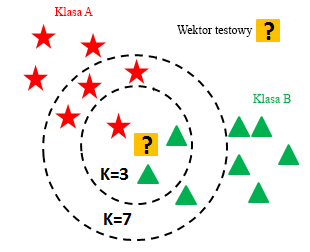
\includegraphics[width=10cm]{Obrazy/klasyfikacjaKNN.jpg}
        \caption{Przykład klasyfikacji KNN~\cite{KNNObraz}.}
        \label{fig.klasyfikacjaKNN}
    \end{figure}

    Na rysunku~\ref{fig.klasyfikacjaKNN} wyróżnione są wektory ze zbioru uczącego należące do klasy ,,A'' oraz klasy
    ,,B''. Ponadto na środku rysunku~\ref{fig.klasyfikacjaKNN} znajduje się wektor, który ma zostać
    sklasyfikowany do jednej z wyżej wymienionych klas.
    Dla parametru ,,k'' równego 3 wektor testowy zostanie przypisany do klasy ,,B'', gdyż z trzech najbliższych wektorów dwa
    należą do klasy ,,B''. W przypadku, gdy parametr ,,k'' będzie równy 7 wektor testowy zostanie przypisany do klasy
    ,,A''. Spośród siedmiu najbliższych sąsiadów, cztery wektory należą do klasy ,,A'', natomiast trzy - do klasy ,,B''.

    Wybór parametru $k$ jest zależny od rodzaju danych. Im większa wartość $k$, tym mniejszy wpływ na proces
    klasyfikacji ma szum, który określa błędne dane w zbiorze uczącym. Istnieją metody dobierające optymalną wartość $k$ dla
    danego zbioru uczącego. Do jednej z nich należy optymalizacja hiperparametryczna.

    Na końcu sekcji~\ref{subsec:zastosowanie-w-projekcie} został przedstawiony sposób, w jaki generowany jest zbiór
    uczący.
    Szacowanie wieku metodą KNN w pierwszym kroku polega na stworzeniu wektoru, który został opisany
    wzorem~\ref{wzor.hogKnn}.
    Następnym krokiem jest przydzielenie danego wektoru do klasy (wieku).

    \chapter{Badania}\label{ch:badania}
    W niniejszym rozdziale zostaną przedstawione badania metody bazowej oraz jej modyfikacji.
    Sekcja ~\ref{sec:środowisko-pracy} prezentuje środowisko pracy, a dokładniej mówiąc wszystkie
    niezbędne narzędzia i akcesoria, które pozwoliły skutecznie przeprowadzić badania. Ponadto zaprezentowana jest
    metodyka badań oraz statystyki z działania programu.
    Sekcja~\ref{sec:wykrywanie-krawędzi-przez-detektor-canny} ukazuje efekty wykrywania zmarszczek przez detektor
    Canny.
    Sekcja~\ref{sec:skuteczność-poszczególnych-metod-szacowania-wieku} zawiera porównanie metody bazowej oraz jej
    modyfikacji
    pod kątem skuteczności szacowania wieku.

    \section{Środowisko, metodyka badań oraz statystyki z działania algorytmów}\label{sec:środowisko-pracy}

    W celu przeprowadzenia badań do niniejszej pracy magisterskiej wymagane było stworzenie programu,
    który wykrywa twarz oraz wyodrębnia cechy z twarzy. Wyżej wymieniony program został napisany w języku Java.
    Biblioteka, która pomogła wyodrębniać cechy z obrazu, to OpenCv. Sama ta biblioteka jest stworzona w języku C++, jednak
    istnieją jej modyfikacje, które zostały napisane w innych językach. Najczęściej spotykane są modyfikacje
    stworzone w języku Java oraz Python. Ponadto w Javie generowano dane dla metody bazowej oraz wszystkich
    jej modyfikacji. Dodatkowo to w tym języku zrealizowano szacowanie wieku we wszystkich metodach, z
    pominięciem metody, która stosuje algorytm KNN (sekcja~\ref{sec:metoda-hog-oraz-algorytm-knn}).

    Grupowanie danych algorytmem Fuzzy C-means zostało zrealizowane za pomocą programu Matlab.
    Również szacowanie wieku dla metody stosującej algorytm KNN przeprowadzono za pomocą wyżej wymienionego
    programu.

    Dane z treningu były generowane do plików CSV oraz JSON. Ponadto większość kluczowych operacji była logowana do plików. Do
    tego celu posłużyła popularna biblioteka Log4j.
    Generacja plików JSON była zrealizowana przez bibliotekę GSON z pakietu com.google.code.gson, natomiast
    do generacji plików CSV nie została wykorzystana zewnętrzna biblioteka.

    W pracy została odtworzona oryginalna praca autorów, która
    będzie dalej nazywana metodą bazową.
    W celu poprawienia wyników metody bazowej wprowadzono kilka modyfikacji, a
    w kolejnym kroku wyniki zostały porównane z pozostałymi metodami.

    Do oceny skuteczności szacowania wieku za pomocą poszczególnych metod potrzebna jest baza treningowa oraz testowa.
    Baza testowa może pochodzić od części danych treningowych. Istnieje kilka metod rozdzielenia jednej bazy na bazę
    treningową oraz testową.
    Jedną z nich jest rozdzielenie bazy w oparciu o stosunek. Oznacza, to, że uzyskany zbiór treningowy będzie wynosił
    $x$ procent np. 90\%, a zbiór testowy odpowiednio $100\% -x$, np 10\%~\cite{dataMiningAlgorithms}.

    Drugi ze sposobów to schemat CV-n, zwany również walidacją krzyżową.
    Zakłada ona, że zbiór danych zostanie podzielony na n równych podzbiorów.
    Następnie wykonuje się n iteracji. W każdej iteracji jeden podzbiór zostaje zbiorem testowym, natomiast reszta
    podzbiorów tworzy zbiór treningowy.
    Każda iteracja daje wynik działania klasyfikatora; w przypadku niniejszej pracy jest to
    MAE (ang. mean absolute error), który określa średni błąd bezwzględny.
    \large
    \begin{equation}
        MAE = \frac{\sum_{i=1}^{n}\left | R_{i}-P_{i} \right |}{n}
        \label{wzor.mae}
    \end{equation}
    \normalsize
    gdzie $R_{i}$ oznacza wartość rzeczywistą wieku dla i-tego zdjęcia, $n$ oznacza liczbę zdjęć testowych.
    Natomiast $P_{i}$ oznacza wartość szacowaną wieku.
    W wyniku n iteracji otrzymuje się uśredniony wynik działania klasyfikatora.\cite{dataMiningAlgorithms}.
    Najczęściej dokonuje się tego przez wyliczenie średniej wartości n rezultatów uzyskanych po przeprowadzeniu
    n iteracji.

    Metoda Leave-One-Out zakłada wykluczenie jednego obiektu, który reprezentuje zbiór testowy. Natomiast reszta obiektów zostaje zakwalifikowana do zbioru treningowego.
    Po przetestowaniu klasyfikatora powyższym obiektem otrzymuje się wynik skuteczności klasyfikacji. Proces ten jest powtarzany dla wszystkich obiektów.
    Metoda Leave-One-Out działa dokładnie tak samo jak metoda CV-n dla $n$ równego liczbie obiektów
    w zbiorze danych.\cite{dataMiningAlgorithms}

    Dla każdej metody dokonano porównania 257 zdjęć, co stanowi 10\% ogólnej liczby obrazów biorących udział w
    badaniach, natomiast pozostałe 90\% obrazów brało udział w analizie danych, jako zbiór treningowy dla każdej metody
    szacowania wieku.
    Ponadto sprawdzono jakość klasyfikatora stosując metodę walidacji krzyżowej. Najczęściej w walidacji krzyżowej
    parametr $n$ wynosi 5.

    %    natomiast każda z nich miała zmieniane parametry algorytmów. W przypadku metody z algorytmem grupowania Fuzzy C-means zmianie
    %    podlegały parametry tego właśnie algorytmu. Analogicznie zmieniano właściwości odpowiednich algorytmów dla metody HOG i klasyfikatora KNN.

    \subsection*{Baza zdjęć oraz statystyki z działania programu}
    Baza UTKface zawiera 23708 zdjęć.
    Nazwa każdego obrazu zawiera informację odnośnie wieku, płci i rasy fotografowanej osoby, podane w tej kolejności.
    Fotografie zebrane w bazie przedstawiają osoby w wieku od 1 do 116 lat.

    Detektor twarzy był w stanie wyznaczyć obszar twarzy dla 14583 obrazów.
    Na pozostałych zdjęciach twarz nie została wykryta z różnych przyczyn. Część z tych zdjęć nie przedstawiała całej
    twarzy lub twarz była na nich częściowa przysłonięta. W niektórych przypadkach problem stanowiło złe oświetlenie
    sfotografowanej twarzy lub słaba jakość obrazu.
    Jednak spośród 14583 obrazów tylko 2574 brało udział w liczeniu zmarszczek, ponieważ jedynie w tej grupie algorytm
    poprawnie wykrył obszar nosa oraz oczu, które są niezbędne do dalszych obliczeń. Podobnie jak w przypadku braku
    identyfikacji twarzy, wśród przyczyn można wymienić złe oświetlenie twarzy, słabą jakość obrazu albo złe
    ustawienie twarzy względem obiektywu.

    Średni czas generacji współczynnika zmarszczek dla obrazu po wykryciu twarzy wyniósł 0,467 sekundy dla metody
    bazowej.
    Dla metody, w której została odjęta strefa druga, generacja trwała 0,465 sekund,
    dla metody HOG 0,543 sekundy, natomiast dla metody HOG wraz z klasyfikacją KNN - 0,543 sekundy.
    %todo wplyw przerwa... jakich przerwan... ja bym to zostawil i jak sie doczepi to doprecyzuje...
    Powyższe dane wykazują, że najszybciej wskaźnik zmarszczek był generowany przez algorytm metody
    po odjęciu jednej strefy.

    Warto porównać również szybkość szacowania wieku na podstawie danego współczynnika zmarszczek.
    Średni czas szacowania wieku dla danego obrazu wyniósł 0,585 sekundy dla metody bazowej.
    Dla metody, w której została
    odjęta strefa druga, ten czas wyniósł 0,583 sekundy, a dla metody HOG 0,675 sekundy.
    Szacowanie wieku dla metody HOG wraz z klasyfikacją KNN przeprowadził
    program realizowany przez skrypt w Matlabie, więc nie porównano szybkości działania
    algorytmu zaimplementowanego w Matlabie do algorytmu zaimplementowanego w Javie.
    Reasumując - najszybciej szacował wiek algorytm zawierający odjętą strefę.


    %Skad wzielismy dane testowe
    %porownanie metod testowych
    %http://edu.pjwstk.edu.pl/wyklady/adn/scb/wyklad9/w9.htm
    %    Wstep jakie metody porownano i co tam zmieniano
    \section{Wykrywanie zmarszczek}\label{sec:wykrywanie-krawędzi-przez-detektor-canny}
    W tej sekcji zostaną przedstawione typowe problemy napotkane podczas detekcji zmarszczek metodą Canny oraz Histogram
    of Oriented Gradients.
    W wielu zdjęciach wystąpiły nieprawidłowe detekcje zmarszczek.

    Krawędzie związane tylko ze zmarszczkami są widoczne na obrazie~\ref{fig.dobryRyjek}
    \begin{figure}
        \centering
        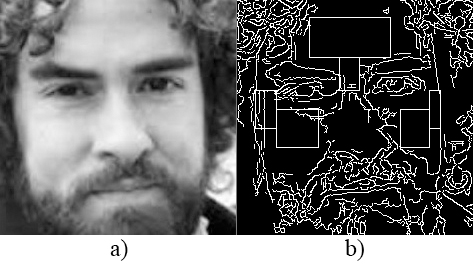
\includegraphics[width=11cm]{Obrazy/dobryRyjekWszystkieStrefyGray.jpg}
        \captionsetup{justification=centering}
        \caption{Przykład prawidłowej detekcji zmarszczek. \newline
        a) Obraz przed detekcją zmarszczek b) Obraz po detekcji zmarszczek}
        \label{fig.dobryRyjek}
    \end{figure}
    Obraz~\ref{fig.dobryRyjek} będzie dobrym punktem odniesienia do przypadków błędnych detekcji zmarszczek.
    %todo - ogolnie zrobic na sam koniec sprawdzenie czy nie ma rozjazdow z obrazami
    Pierwszym przykładem jest wykrycie krawędzi związanych z brwiami. Na obrazie~\ref{fig.zlyRyjek} można zauważyć,
    że ilość krawędzi w strefie 2 jest duża i nie identyfikują one zmarszczek.
    \begin{figure}
        \centering
        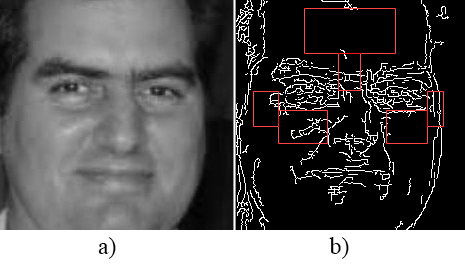
\includegraphics[width=11cm]{Obrazy/brwi.png}
        \captionsetup{justification=centering}
        \caption{Przykład nieprawidłowej detekcji zmarszczek w strefie 2. \newline
        a) Obraz przed detekcją zmarszczek b) Obraz po detekcji zmarszczek }
        \label{fig.zlyRyjek}
    \end{figure}
    Z bazy zdjęć wyselekcjonowano 20 obrazów, na których zmarszczki zostały wykryte poprawnie, oraz 20 kolejnych
    obrazów, gdzie
    detekcja zmarszczek została zaburzona przez brwi nachodzące na strefę 2. Aby uzyskać możliwie miarodajne i
    uśrednione wyniki tego eksperymentu, wybrano fotografie osób w wieku od 24 do 38 lat, ponieważ w tym wieku
    zmarszczki na twarzy są zauważalne, ale nie za bardzo głębokie.
    Dla każdego obrazu wyliczono współczynnik zmarszczek ze strefy 2. Następnie dla obu grup wyliczono średnią oraz
    odchylenie standardowe współczynnika zmarszczek. W tabeli~\ref{tab.brwi} przedstawiono wyniki powyższych badań
    dla detektora Cannego, natomiast w tabeli~\ref{tab.brwiHog} przedstawiono wyniki badań dla detekcji zmarszczek
    algorytmem HOG-a.
    \begin{table}[h!]
        \centering
        \caption{Eksperyment 1: wykrywanie zmarszczek w strefie 2 dla detektora Canny.}
        \begin{tabular}{|M{5cm}|M{4cm}|M{5cm}|}
            \hline
            & \begin{tabular}[c]{@{}c@{}}
                  Obrazy\\ze zmarszczkami \\wykrytymi prawidłowo
            \end{tabular} &
            \begin{tabular}[c]{@{}c@{}}
                Obrazy\\ze zmarszczkami \\wykrytymi nieprawidłowo
            \end{tabular} \\ \hline
            Średnia współczynnika zmarszczek & 0,05 & 0,061                                                                                      \\ \hline
            Odchylenie standardowe współczynnika zmarszczek & 0,009
            & 0,011                                                                                      \\ \hline
        \end{tabular}
        \label{tab.brwi}
    \end{table}
    W wyniku przeprowadzenia eksperymentu 1 dla detektora Canny uzyskano współczynnik zmarszczek równy 0,05 oraz
    odchylenie standardowe 0,009 dla
    obrazów ze zmarszczkami
    wykrytymi prawidłowo, natomiast brwi nachodzące na strefę 2 spowodowały zwiększenie współczynnika zmarszczek do
    0,061, natomiast odchylenie standardowe wyniosło 0,011.
    Zauważona różnica nie jest jednak na tyle wysoka, by móc wyraźnie stwierdzić, że będzie miała istotny wpływ na
    szacowanie wieku.
    \begin{table}[h!]
        \centering
        \caption{Eksperyment 1: wykrywanie zmarszczek w strefie 2 dla detektora HOG-a.}
        \begin{tabular}{|M{5cm}|M{4cm}|M{5cm}|}
            \hline
            & \begin{tabular}[c]{@{}c@{}}
                  Obrazy\\ze zmarszczkami \\wykrytymi prawidłowo
            \end{tabular} &
            \begin{tabular}[c]{@{}c@{}}
                Obrazy\\ze zmarszczkami \\wykrytymi nieprawidłowo
            \end{tabular} \\ \hline
            Średnia współczynnika zmarszczek & 2,512
            & 2,562
            \\ \hline
            Odchylenie standardowe współczynnika zmarszczek & 0,027
            & 0,050
            \\ \hline
        \end{tabular}
        \label{tab.brwiHog}
    \end{table}
    W przypadku HOG dla prawidłowo wykrytych zmarszczek średnia współczynnika zmarszczek wyniosła 2,512, natomiast
    odchylenie standardowe 0,027. Dla nieprawidłowo wykrytych zmarszczek średnia współczynnika zmarszczek zwiększyła
    się do 2,562, natomiast odchylenie standardowe wyniosło 0,050.
    Podobnie jak w przypadku detektora Cannego nie jest jasne, czy różnice mają wpływ na jakość szacowania wieku.
    %    Trzeba wziąć więcej obrazów. Zrobić grupę obrazów, gdzie brwi wchodzą w region i drugą grupę
    %    (o tej samej liczbie obrazów), w której nie ma tego problemu. Dla każdego obrazu policzyć parametry.
    %    Potem dla każdej grupy policzyć średnią i odchylenie standardowe. I zobaczyć na wykresie czy średnia
    %    +/- odchylenie z jednej grupy pokrywa wartości dla średnia +/- odchylenie z drugiej grupy.
    %    Najlepiej byłoby jakby te zakresy nie naszły na siebie.
    %    - to wtedy statystycznie wynik można traktować jako pewny. Jak Pan nie ma tyle danych, to proszę
    %    we wnioskach najwyżej napisać, że danych jest trochę za mało, ale widoczna jest tendencja
    %    (o ile ona wyjdzie z obliczeń).

    Kolejnym problemem okazała się grzywka nachodząca na obszar strefy 1.
    Na obrazie~\ref{fig.grzywka} można zauważyć wykryte krawędzie,
    które identyfikują włosy.
    \begin{figure}[hb]
        \centering
        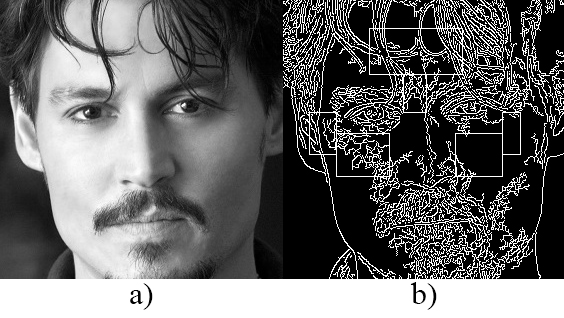
\includegraphics[width=11cm]{Obrazy/zlyRyjekZGrzywka.jpg}
        \captionsetup{justification=centering}
        \caption{Przykład nieprawidłowej detekcji zmarszczek w strefie 1. \newline
        a) Obraz przed detekcją zmarszczek b) Obraz po detekcji zmarszczek }
        \label{fig.grzywka}
    \end{figure}
    Podobnie jak powyżej, przeprowadzono porównanie,
    które ma na celu sprawdzenie wpływu nieprawidłowo wykrytych krawędzi na współczynnik zmarszczek.
    Do wspomnianego celu obliczono średni współczynnik zmarszczek oraz odchylenie standardowe ze strefy 1 dla osób w
    wieku od 24 do 38 lat. W tym eksperymencie wykorzystano 20 obrazów z poprzedniego eksperymentu, na których
    zmarszczki zostały wykryte poprawnie, oraz 20 kolejnych zdjęć, gdzie grzywka nachodząca na strefę 1
    spowodowała nieprawidłowe wykrycie zmarszczek. Wyniki detekcji detektorem Cannego zaprezentowano w
    tabeli~\ref{tab.grzywka}, natomiast wyniki dla algorytmu HOG-a pokazano w tabeli~\ref{tab.grzywkaHog}
    \begin{table}[h!]
        \centering
        \caption{Eksperyment 2: wykrywanie zmarszczek w strefie 1 za pomocą detektora Canny.}
        \begin{tabular}{|M{5cm}|M{4cm}|M{5cm}|}
            \hline
            & \begin{tabular}[c]{@{}c@{}}
                  Obrazy\\ze zmarszczkami \\wykrytymi prawidłowo
            \end{tabular} &
            \begin{tabular}[c]{@{}c@{}}
                Obrazy\\ze zmarszczkami \\wykrytymi nieprawidłowo
            \end{tabular} \\ \hline
            Średnia współczynnika zmarszczek & 0,056
            & 0,079                                                                                      \\ \hline
            Odchylenie standardowe współczynnika zmarszczek & 0,01
            & 0,014                                                                                      \\ \hline
        \end{tabular}
        \label{tab.grzywka}
    \end{table}
    Średnia współczynnika zmarszczek dla prawidłowo wykrytych zmarszczek, dla strefy 1 w eksperymencie nr 2 wyniosła
    0,056, natomiast odchylenie standardowe było równe 0,01. Grzywka nachodząca na strefę 1 zwiększyła
    średni współczynnik zmarszczek do 0,079 oraz odchylenie standardowe do 0,014.
    Podobnie, jak we wnioskach po eksperymencie 1, nie można jednoznacznie stwierdzić, czy zwiększony współczynnik o
    0,023 oraz odchylenie standardowe o 0,004 istotnie wpłynie na oszacowany wiek.
    \begin{table}[h!]
        \centering
        \caption{Eksperyment 2: wykrywanie zmarszczek w strefie 1 za pomocą detektora Canny.}
        \begin{tabular}{|M{5cm}|M{4cm}|M{5cm}|}
            \hline
            & \begin{tabular}[c]{@{}c@{}}
                  Obrazy\\ze zmarszczkami \\wykrytymi prawidłowo
            \end{tabular} &
            \begin{tabular}[c]{@{}c@{}}
                Obrazy\\ze zmarszczkami \\wykrytymi nieprawidłowo
            \end{tabular} \\ \hline
            Średnia współczynnika zmarszczek & 2,569
            & 2,617
            \\ \hline
            Odchylenie standardowe współczynnika zmarszczek &0,041
            & 0,056
            \\ \hline
        \end{tabular}
        \label{tab.grzywkaHog}
    \end{table}
    W strefie 1 średni współczynnik zmarszczek dla obrazów zawierających prawidłowo wykryte zmarszczki wyniósł 2,569,
    natomiast odchylenie standardowe 0,041. Dla obrazów, gdzie detekcja dała nieprawidłowy wynik, średnia wartość
    współczynnika wyniosła 2,617, a odchylenie standardowe było równe 0,056.
    Podobnie jak w przypadku detekcji metodą Canny, nie jest możliwe jednoznaczne stwierdzenie, czy zauważona
    tendencja istotnie zafałszuje szacowany wiek.
    \section{Skuteczność poszczególnych metod szacowania wieku}\label{sec:skuteczność-poszczególnych-metod-szacowania-wieku}
    W niniejszej sekcji zaprezentowano jakość szacowania wieku przez algorytm bazowy oraz jego modyfikację. W każdej
    metodzie zaprezentowano wyniki z testowania za pomocą schematu CV oraz podziału na zbiór treningowy i testowy w
    stosunku 90\% do 10\%.
    \subsection{Metoda bazowa}\label{subsec:metoda-bazowa}
    Jako pierwsza została przetestowana metoda bazowa.
    Sprawdzono dokładność szacowania wieku zmieniając parametry algorytmu trenującego Fuzzy C-means:
    \begin{itemize}
        \item m - współczynnik rozmycia
        \item g - ilość grup
        \item $\epsilon$ - kryterium (wzór~\ref{wzor.koniecIteracjiWarunek})
    \end{itemize}
    Ponadto warto wspomnieć, że detektor Canny używany przy detekcji zmarszczek posiadał niezmienne wartości progu
    $T_{l} = 10$ oraz $T_{h} = 100$ podczas prowadzenie badań.
    Przykładowy wynik testowania metody został przedstawiony w tabeli~\ref{tab.przykladoweWyniki}

    \begin{table}[h]
        \centering
        \caption{Przykładowy wynik testowania zawierający 15 wyników.}
        \label{tab.przykladoweWyniki}
        \begin{tabular}{|M{2cm}|M{2cm}|M{2cm}|}
            \hline
            \begin{tabular}[c]{@{}c@{}}
                wiek\\   prawdziwy
            \end{tabular} & wiek wykryty & różnica \\ \hline
            10 & 25 & 15      \\ \hline
            15 & 26 & 11      \\ \hline
            20 & 31 & 11      \\ \hline
            25 & 15 & 10      \\ \hline
            30 & 45 & 15      \\ \hline
            35 & 48 & 13      \\ \hline
            40 & 26 & 14      \\ \hline
            45 & 49 & 4       \\ \hline
            50 & 58 & 8       \\ \hline
            55 & 34 & 21      \\ \hline
            60 & 50 & 10      \\ \hline
            65 & 80 & 15      \\ \hline
            70 & 65 & 5       \\ \hline
            75 & 80 & 5       \\ \hline
            80 & 67 & 13      \\ \hline
        \end{tabular}
    \end{table}
    \subsection*{Wyniki z testowania 10\% zdjęć}
    Badania rozpoczęto od przeprowadzenia testu z następującymi parametrami wejściowymi algorytmu FCM:
    \begin{itemize}
        \item m = 2,0,
        \item n = 1000,
        \item g = 10,
        \item $\epsilon$=1e-5.
    \end{itemize}
    W kolejnych krokach badań zmieniano jeden z parametrów FCM, jednocześnie zachowując stałe wartości pozostałych
    parametrów.
    Tabela~\ref{tab.bazowa_m} przedstawia, jak zmieniała się wartość MAE w zależności od zmian parametru m.
    W kolejnej tabeli~\ref{tab.bazowa_e} przedstawiono wyniki przy
    zmianie parametru $\epsilon$.
    W tabeli~\ref{tab.bazowa_g} przedstawiono
    jakość szacowania
    wieku przy modyfikacji parametru g.
    \begin{table}[h!]
        \centering
        \caption{Wpływ parametru m na wartość MAE w metodzie bazowej.}
        \begin{tabular}{|c|c|c|c|}
            \hline
            & m=2,0 & m=3,0 & m=5,0 \\ \hline
            MAE & 12,79 & 11,25 & 11,68 \\ \hline
        \end{tabular}
        \label{tab.bazowa_m}
    \end{table}
    \begin{table}[h!]
        \centering
        \caption{Wpływ parametru $\epsilon$ na MAE w metodzie bazowej.}
        \begin{tabular}{|c|c|c|c|}
            \hline
            & $\epsilon=1e-6$ & $\epsilon=1e-7$ & $\epsilon=1e-8$ \\ \hline
            MAE & 11,18 & 11,3 & 11,34 \\ \hline
        \end{tabular}
        \label{tab.bazowa_e}
    \end{table}
    \begin{table}[h!]
        \centering
        \caption{Wpływ parametru $g$ na wynik MAE w metodzie bazowej.}
        \begin{tabular}{|c|c|c|c|}
            \hline
            & $g=20$ & $g=50$ & $g=100$ \\ \hline
            MAE & 10,99 & 10,76 & 10,98 \\ \hline
        \end{tabular}
        \label{tab.bazowa_g}
    \end{table}

    Najlepszy wynik MAE dla modyfikacji parametru m, osiągnięto dla m=3,0. Zwiększenie parametru m z 2,0 do 3,0
    znacznie poprawiło jakość szacowania wieku.
    Zwiększanie parametru $\epsilon$ nie miało znacznego wpływu na jakość szacowania wieku.
    Zmiana liczby grup z 20 do 50 nieznacznie polepszyła MAE. Ponadto widać, że dalsze zwiększanie liczby grup nie
    wpływa na wynik MAE.

    Metoda oryginalna uzyskała najlepszą jakość szacowania wieku dla następujących parametrów:
    \begin{itemize}
        \item m=2,0
        \item n=1000
        \item $\epsilon=1e-5$
        \item g=20
    \end{itemize}
    Dla tych parametrów MAE osiągnęło 10,76.

    \subsection*{Wyniki z walidacji krzyżowej CV-5}
    Badania dla walidacji krzyżowej miały taki sam przebieg, jak w przypadku procesu testowania 10\% zdjęć.
    Zmieniano parametr m (tabela~\ref{tab.bazowa_m_cv}), $\epsilon$ (tabela~\ref{tab.bazowa_e_cv})
    oraz g (tabela~\ref{tab.bazowa_g_cv}).
    \begin{table}[h!]
        \centering
        \caption{Wpływ parametru m na wartość MAE w metodzie bazowej.}
        \begin{tabular}{|c|c|c|c|}
            \hline
            & m=2,0 & m=3,0 & m=5,0 \\ \hline
            MAE & 8,64 & 8,64 & 9,07 \\ \hline
        \end{tabular}
        \label{tab.bazowa_m_cv}
    \end{table}
    \begin{table}[h!]
        \centering
        \caption{Wpływ parametru $\epsilon$ na MAE w metodzie bazowej.}
        \begin{tabular}{|c|c|c|c|}
            \hline
            & $\epsilon=1e-6$ & $\epsilon=1e-7$ & $\epsilon=1e-8$ \\ \hline
            MAE & 8,64 & 8,64 & 8,64 \\ \hline
        \end{tabular}
        \label{tab.bazowa_e_cv}
    \end{table}
    \begin{table}[h!]
        \centering
        \caption{Wpływ parametru $g$ na wynik MAE w metodzie bazowej.}
        \begin{tabular}{|c|c|c|c|}
            \hline
            & $g=20$ & $g=50$ & $g=100$ \\ \hline
            MAE & 8,6 & 8,53 & 8,58 \\ \hline
        \end{tabular}
        \label{tab.bazowa_g_cv}
    \end{table}
    Zmiana parametru m z wartości 2,0 do 5,0 znacząco pogorszyła MAE. Modyfikacja parametru $\epsilon$ nie wpłynęła
    na wartość MAE, natomiast zwiększenie jakości szacowania wieku nastąpiło przy zwiększeniu grupy z 10 do 20.
    Największa jakość szacowania wieku została osiągnięta dla następującej kombinacji parametrów wejściowych:
    \begin{itemize}
        \item m=2,0;
        \item g=20
        \item n=1000
        \item $\epsilon=1e-5$
    \end{itemize}
    Dla powyższej kombinacji parametrów FCM, MAE osiągnęło 8,58 roku.
    Testowanie za pomocą walidacji krzyżowej pokazało, że MAE ma znacznie lepszą wartość, niż w przypadku testów ,,10\%
    zdjęć''.
    %parametry takie i takie i jakie wyniki daly zmiany o ile procent sie polepszyl lub pogorszyl MAE

    \subsection{Odjęcie strefy 2}\label{subsec:odjęcie-strefy-2}
    \subsection*{Wyniki z testowania 10\% zdjęć}
    W kolejnym kroku została przetestowana metoda, które nie uwzględnia zmarszczek ze strefy 2.
    Podobnie jak w sekcji~\ref{subsec:metoda-bazowa} wykonywano testy dla takich samych parametrów algorytmu Fuzzy
    C-means.
    Tabela~\ref{tab.odjeta_m} przedstawia, jak zmieniała się wartość MAE w zależności od zmian parametru m.
    W kolejnej tabeli~\ref{tab.odjeta_e} przedstawiono wyniki przy
    zmianie parametru $\epsilon$.
    W tabeli~\ref{tab.odjeta_g} przedstawiono
    jakość szacowania
    wieku przy modyfikacji parametru g.
    \begin{table}[h!]
        \centering
        \caption{Wpływ parametru m na wartość MAE w metodzie po odjęciu strefy 2.}
        \begin{tabular}{|c|c|c|c|}
            \hline
            & m=2,0 & m=3,0 & m=5,0 \\ \hline
            MAE & 13,78 & 13,94 & 14,31 \\ \hline
        \end{tabular}
        \label{tab.odjeta_m}
    \end{table}
    \begin{table}[h!]
        \centering
        \caption{Wpływ parametru $\epsilon$ na MAE w metodzie po odjęciu strefy 2.}
        \begin{tabular}{|c|c|c|c|}
            \hline
            & $\epsilon=1e-6$ & $\epsilon=1e-7$ & $\epsilon=1e-8$ \\ \hline
            MAE & 13,75 & 13,97 & 12,42 \\ \hline
        \end{tabular}
        \label{tab.odjeta_e}
    \end{table}
    \begin{table}[h!]
        \centering
        \caption{Wpływ parametru $g$ na wynik MAE w metodzie po odjęciu strefy 2.}
        \begin{tabular}{|c|c|c|c|}
            \hline
            & $g=20$ & $g=50$ & $g=100$ \\ \hline
            MAE & 13,82 & 13,91 & 13,74 \\ \hline
        \end{tabular}
        \label{tab.odjeta_g}
    \end{table}

    Zwiększanie parametru wejściowego m pogarszało wyniki szacowania wieku, natomiast poprawa wyników nastąpiła przy
    zmniejszeniu $\epsilon$ do wartości $1e-8$. Liczba grup nie miała większego wpływu na MAE.
    Dla parametrów FCM:
    \begin{itemize}
        \item m=2;
        \item g=10
        \item n=1000
        \item $\epsilon=1e-8$
    \end{itemize}
    osiągnięto najlepszą wartość MAE równą 12,42 roku.

    \subsection*{Wyniki walidacji krzyżowej CV-5}

    Podobnie, jak w testowaniu za pomocą 10\% zdjęć zbadano wpływ parametrów:
    \begin{itemize}
        \item m (tabela~\ref{tab.odjeta_m_cv})
        \item $\epsilon$ (tabela~\ref{tab.odjeta_e_cv})
        \item g (tabela~\ref{tab.odjeta_g_cv})
    \end{itemize}

    \begin{table}[h!]
        \centering
        \caption{Wpływ parametru m na wartość MAE w metodzie po odjęciu strefy 2.}
        \begin{tabular}{|c|c|c|c|}
            \hline
            & m=2,0 & m=3,0 & m=5,0 \\ \hline
            MAE & 10,74 & 11,03 & 11,23 \\ \hline
        \end{tabular}
        \label{tab.odjeta_m_cv}
    \end{table}
    \begin{table}[h!]
        \centering
        \caption{Wpływ parametru $\epsilon$ na MAE w metodzie po odjęciu strefy 2.}
        \begin{tabular}{|c|c|c|c|}
            \hline
            & $\epsilon=1e-6$ & $\epsilon=1e-7$ & $\epsilon=1e-8$ \\ \hline
            MAE & 10,94 & 10,94 & 10,94 \\ \hline
        \end{tabular}
        \label{tab.odjeta_e_cv}
    \end{table}
    \begin{table}[h!]
        \centering
        \caption{Wpływ parametru $g$ na wynik MAE w metodzie po odjęciu strefy 2.}
        \begin{tabular}{|c|c|c|c|}
            \hline
            & $g=20$ & $g=50$ & $g=100$ \\ \hline
            MAE & 10,9 & 11,01 & 11,03 \\ \hline
        \end{tabular}
        \label{tab.odjeta_g_cv}
    \end{table}

    Podobnie jak przy testowaniu 10\% zdjęć, zwiększanie parametru wejściowego m pogarszało wyniki szacowania wieku.
    Zwiększenie $\epsilon$ z $1e-5$ do $1e-6$ minimalnie pogorszyło wyniki. Dalsze zwiększanie tego parametru
    pozwoliło uzyskać identyczne MAE równe 10,94 roku.
    Liczba grup nie miała większego wpływu na MAE.
    Dla poniższych parametrów FCM:
    \begin{itemize}
        \item m=2;
        \item g=10
        \item n=1000
        \item $\epsilon=1e-5$
    \end{itemize}
    osiągnięto najlepszą wartość MAE równą 10,74 roku.

    W porównaniu do metody bazowej szacowanie wieku jest znacznie gorsze. Odjęcie jednej strefy powoduje utratę
    danych o zmarszczkach i zwiększa błąd szacowania wieku.

    \subsection{Metoda HOG}\label{subsec:metoda-hog}
    Kolejną przetestowaną modyfikacją była ta w której użyto algorytmu HOG.
    Podobnie jak w sekcjach~\ref{subsec:odjęcie-strefy-2} oraz~\ref{subsec:metoda-bazowa} modyfikowano parametry
    algorytmu Fuzzy C-means, jednak dodatkowo dokonano zmiany parametru HOG, Parametrem poddanym modyfikacji był
    rozmiar komórki. Najpierw ustalono wymiary komórki na 3x3 pikseli, następnie na 6x6 pikseli, a na końcu 9x9
    pikseli.
    Rozmiar bloku dla wszystkich modyfikacji rozmiaru komórek wyniósł
    2x2 komórki. Liczba kubełków histogramu była stała i wynosiła 9 dla wszystkich pomiarów.
    \subsection*{Wyniki z testowania 10\% zdjęć}
    W pierwszym teście ustalono parametry Fuzzy C-means: m = 2,0, n = 100 oraz g = 10, n = 100
    oraz $\epsilon$ = 1e-5.
    Wpływ parametru m oraz rozmiarów komórki na MAE jest przedstawiony w tabeli~\ref{tab.hog}
    \begin{table}[h!]
        \centering
        \caption{Wpływ parametru m oraz rozmiarów komórki na MAE.}
        \begin{tabular}{|c|c|c|c|}
            \hline
            m=2,0 & m=3,0 & m=5,0 &                     \\ \hline
            16,65 & 16,92 & 11,68 & komórka 3x3 piksele \\ \hline
            16,48 & 16,78 & 11,3 & komórka 6x6 piksele \\ \hline
            11,99 & 16,89 & 11,32 & komórka 9x9 piksele \\ \hline
        \end{tabular}
        \label{tab.hog}
    \end{table}
    Rozmiary komórki 3x3 oraz 6x6 pikseli przy zmianach parametru m wprowadzają niewielkie zmiany w jakości
    szacowania wieku. Zmiana rozmiaru komórki na 9x9 pikseli wprowadza duża zmianę wartości MAE. Wartość ta,
    zmniejsza się drastycznie do około 11,3 roku.

    Następnie badano wpływ parametru $\epsilon$ (tabela~\ref{tab.hog1}).
    \begin{table}[h!]
        \centering
        \caption{Wpływ parametru $\epsilon$ oraz rozmiarów komórki na MAE.}
        \begin{tabular}{|c|c|c|c|}
            \hline
            $\epsilon=1e-6$ &  $\epsilon=1e-7$ &  $\epsilon=1e-8$ &                     \\ \hline
            16,79 & 16,99 & 16,7 & komórka 3x3 piksele \\ \hline
            16,49 & 16,86 & 16,55 & komórka 6x6 piksele \\ \hline
            11,31 & 11,31 & 11,28 & komórka 9x9 piksele \\ \hline
        \end{tabular}
        \label{tab.hog1}
    \end{table}

    Podobnie jak przy badaniu wpływu parametru m (tabela~\ref{tab.hog}) polepszenie nastąpiło dla komórki o rozmiarze
    9x9 pikseli.

    Badanie wpływu grup na jakość szacowania wieku daje również podobne rezultaty do powyżej zaprezentowanych
    (tabela~\ref{tab.hog2}).
    \begin{table}[h!]
        \centering
        \caption{Wpływ parametru $g$ oraz rozmiarów komórki na MAE.}
        \begin{tabular}{|c|c|c|c|}
            \hline
            $g=20$ & $g=50$ & $g=100$ &                     \\ \hline
            16,59 & 15,48 & 15,49 & komórka 3x3 piksele \\ \hline
            16,78 & 16,17 & 16,55 & komórka 6x6 piksele \\ \hline
            11,28 & 11,3 & 11,28 & komórka 9x9 piksele \\ \hline
        \end{tabular}
        \label{tab.hog2}
    \end{table}

    Warto zauważyć, że dla komórki 3x3 nastąpiła znaczna poprawa MAE przy zwiększeniu liczby grup z 20 do 50.

    Reasumując wyniki badań dla testowania 10\% zdjęć można powiedzieć, że najlepszy rezultat MAE osiągnięto dla
    rozmiarów komórki 9x9. Parametry FCM w niewielkim stopniu wpływały na jakość szacowania wieku, która oscylowała
    od wartości MAE 11,28 do 11,31 roku.
    \subsection*{Wyniki walidacji krzyżowej CV-5}
    Parametr m oraz rozmiar komórki wpływał na parametr MAE w sposób przedstawiony w tabeli~\ref{tab.hog11}
    \begin{table}[h!]
        \centering
        \caption{Wpływ parametru m oraz rozmiarów komórki na MAE.}
        \begin{tabular}{|c|c|c|c|}
            \hline
            m=2,0 & m=3,0 & m=5,0 &                     \\ \hline
            9,81 & 9,78 & 9,9 & komórka 3x3 piksele \\ \hline
            9,93 & 9,9 & 9,85 & komórka 6x6 piksele \\ \hline
            9,95 & 9,92 & 9,83 & komórka 9x9 piksele \\ \hline
        \end{tabular}
        \label{tab.hog11}
    \end{table}

    Badanie wpływu parametru m metodą CV ujawnia niewielki rozrzut wyniku MAE.
    Wartości tych wyników zmieniają się o około 0,1 roku. Warto podkreślić, że wartość MAE jest znacznie mniejsza niż
    przy testowaniu za pomocą 10\% zbioru.

    Wpływ parametru $\epsilon$ przedstawiono w tabeli~\ref{tab.hog12}.
    \begin{table}[h!]
        \centering
        \caption{Wpływ parametru $\epsilon$ oraz rozmiarów komórki na MAE.}
        \begin{tabular}{|c|c|c|c|}
            \hline
            $\epsilon=1e-6$ &  $\epsilon=1e-7$ &  $\epsilon=1e-8$ &                     \\ \hline
            9,81 & 9,81 & 9,81 & komórka 3x3 piksele \\ \hline
            9,93 & 9,93 & 9,93 & komórka 6x6 piksele \\ \hline
            9,95 & 9,95 & 9,95 & komórka 9x9 piksele \\ \hline
        \end{tabular}
        \label{tab.hog12}
    \end{table}

    Podobnie jak przy badaniu wpływu parametru m (tabela~\ref{tab.hog}) rozrzut danych jest niewielki. Warto
    podkreślić, że najlepszy wynik osiągnęła najmniejsza komórka 3x3 piksela. Ponadto zmiana parametru $\epsilon$ dla
    każdego rozmiaru komórek nie wpływała na wartość MAE.

    %    Badanie wpływu grup na jakość szacowania wieku daje również podobne rezultaty do powyżej zaprezentowanych
    %    (tabela~\ref{tab.hog21}).
    Na końcu przetestowano wpływ ilości grup w parametrze FCM.
    Wyniki zaprezentowano w tabeli~\ref{tab.hog21}
    \begin{table}[h!]
        \centering
        \caption{Wpływ parametru $g$ oraz rozmiarów komórki na MAE.}
        \begin{tabular}{|c|c|c|c|}
            \hline
            $g=20$ & $g=50$ & $g=100$ &                     \\ \hline
            9,81 & 9,85 & 11,49 & komórka 3x3 piksele \\ \hline
            9,94 & 10,08 & 11,55 & komórka 6x6 piksele \\ \hline
            9,94 & 11,3 & 11,38 & komórka 9x9 piksele \\ \hline
        \end{tabular}
        \label{tab.hog21}
    \end{table}

    Przy testowaniu wpływu ilości grup widoczna jest tendencja pogarszania się wyników dla każdego rozmiaru komórki
    wraz ze wzrostem ilości grup.

    Reasumując wyniki testowania 10\% zdjęć oraz metodą CV najlepszy wynik MAE został osiągnięty dla komórki 3x3
    piksela oraz dla następujących parametrów FCM:
    \begin{itemize}
        \item m=3,0;
        \item g=10;
        \item n=1000;
        \item $\epsilon=1e-5$
    \end{itemize}

    W porównaniu do poprzedniej modyfikacji polegającej na odjęciu strefy 2 następuje znaczna poprawa MAE.
    Jednak nie osiągnięto tak dobrej jakości szacowania wieku jak w metodzie bazowej.

    \subsection{Metoda HOG + KNN}\label{subsec:metoda-hog-+-knn}
    Ostatnią testowaną metodą była ta, która zawiera algorytm HOG, a do klasyfikacji i szacowania używa algorytmu KNN.
    Zmieniano parametr k dla algorytmu KNN, natomiast dla algorytmu HOG - rozmiary komórki.
    Parametr k był równy 1, 3 oraz 5. Rozmiary komórki miały takie same wartości jak przy badaniach w
    sekcji~\ref{subsec:metoda-hog}.
    Liczba kubełków histogramu była stała i wynosiła 9. Podobnie jak w sekcji~\ref{subsec:metoda-hog} ustalono rozmiary
    bloku 2x2 komórki.
    \subsection*{Wyniki z testowania 10\% zdjęć}
    W tabeli~\ref{tab.hogknn} podsumowano jakość szacowania wieku przy zmianach parametru k oraz dla różnych
    rozmiarów komórek.
    \begin{table}[h!]
        \centering
        \caption{Wpływ parametru k oraz rozmiarów komórki na MAE.}
        \begin{tabular}{|c|c|c|c|}
            \hline
            $k=1$ & $k=3$ & $k=5$ &                     \\ \hline
            11,76 & 11,75 & 11,49 & komórka 3x3 piksele \\ \hline
            10,87 & 10,34 & 10,08 & komórka 6x6 piksele \\ \hline
            10,14 & 10,08 & 9,98 & komórka 9x9 piksele \\ \hline
        \end{tabular}
        \label{tab.hogknn}
    \end{table}
    Dla komórki o rozmiarach 3x3 oraz 9x9 pikseli zwiększanie parametru k poprawiało nieznacznie wartość MAE.
    Najlepsza jakość klasyfikacji została osiągnięta dla komórki o rozmiarach 9x9 piksela i parametru k=5.
    \subsection*{Wyniki walidacji krzyżowej CV-5}

    \begin{table}[h!]
        \centering
        \caption{Wpływ parametru k oraz rozmiarów komórki na MAE.}
        \begin{tabular}{|c|c|c|c|}
            \hline
            $k=1$ & $k=3$ & $k=5$  &                     \\ \hline
            10,77 & 10,79 & 10,54 & komórka 3x3 piksele \\ \hline
            10,06 & 9,95 & 10 & komórka 6x6 piksele \\ \hline
            9,66 & 9,6 & 9,64 & komórka 9x9 piksele \\ \hline
        \end{tabular}
        \label{tab.hogknncv}
    \end{table}

    Tak, jak w poprzednich testach metodą CV, można wywnioskować, że jakość szacowania wieku jest większa.
    Najlepsze wartości MAE są osiągane, dla komórki o rozmiarach 9x9 pikseli. Najlepsza wartość MAE wynosi 9,6 i
    została osiągnięta dla parametru k = 3.
    Metoda opierająca się na algorytmie HOG oraz KNN prezentuje najlepsze wyniki MAE spośród wszystkich modyfikacji
    metody bazowej.
    \chapter{Podsumowanie}\label{ch:podsumowanie}
    Dla metody bazowej zmiany poszczególnych parametrów algorytmu FCM przynosiły nieznaczne zmiany MAE, z wyjątkiem
    jednej próby. Przy parametrach m = 2.0, n = 100 $\epsilon$ = 1e-5 oraz g = 10 MAE wyniósł 12,75 roku. Dla reszty
    parametrów zmiany MAE mieściły się w zakresie od 10,66 do 11,67 roku. Największe polepszenie wskaźnika MAE uzyskano
    przy zmianie parametru g na 20 i więcej. Przy powyższej zmianie wartość MAE spadła poniżej 11 lat.

    Dla modyfikacji, która polegała na odjęciu strefy nr 2 wyniki znacznie się pogorszyły. Modyfikacja parametru m
    pogarszała wskaźnik MAE do wartości od 13,66 do 14,41 roku. Minimalna wartość MAE została osiągnięta dla parametrów
    m = 2.0, n = 1000 $\epsilon$ = 1e-8 oraz g = 10. Warto zaznaczyć, że modyfikacja liczby klastrów nie polepszyła
    MAE tak jak w przypadku testowania metody bazowej.

    W metodzie zawierającej modyfikację z algorytmem HOG przetestowano 27 kombinacji parametrów - 3 razy więcej niż przy
    testowaniu metody bazowej. W porównaniu do metody z odjętą strefą MAE uległo znacznemu pogorszeniu. Dla komórki o
    rozmiarach 3x3 pikseli parametry Fuzzy C-means nie dawały znacznej
    poprawy rezultatów MAE. Wskaźnik MAE osiągał wartości od 15,45 do 16,82 roku. Podobne wartości były osiągane dla
    komórki o rozmiarach 6x6 pikseli. W tym przypadku MAE mieściło się w zakresie od 16,16 do 16,89 roku.

    Ostatnia modyfikacja przyniosła poprawę w porównaniu do metody bazowej.
    Dla rozmiaru komórki 5x5 pikseli oraz dla zmiennego parametru n algorytmu KNN błąd MAE osiągał wartości od 11,38 do
    11,75 roku. Warto zauważyć, że poprawa wskaźnika MAE następowała wraz ze wzrostem parametru n. Zmiana rozmiaru
    komórki na 7x7 polepszyła wskaźnik MAE. Osiągał on wartości od 10,34 do 10,77 roku. W tym przypadku najlepszą
    wartość MAE spośród wszystkich przetestowanych osiągnięto dla wartości n = 3, czyli wartości pośredniej.
    Najlepsze wartości osiągnięto dla komórki o rozmiarach 9x9 pikseli. Minimalną i zarazem najlepszą dla wszystkich testów wartość
    osiągnięto dla parametru n = 5.

    Testowanie metody bazowej oraz jej modyfikacji wykazało, że wskaźnik MAE oscylował w granicach 10 lat. Nie jest
    to wartość zadowalająca, gdyż w literaturze ten wskaźnik osiągał wartości około 5 lat. \cite{khryashchevGanin}
    Natomiast udało się polepszyć algorytm bazowy. Modyfikacja zawierająca algorytm HOG oraz KNN poprawiła MAE z 10,66 do
    9,97 roku. W celu poprawy wyników należałoby zwiększyć bazę treningową. Z ponad 20000 obrazów zamieszczonych w bazie tylko 2574
    brało udział w treningu. Wiele zdjęć zostało odrzuconych z powodu braku rozpoznania przez detektor oczu oraz nosa. W
    związku z powyższym należałoby użyć lepszych detektorów lub znaleźć bazę, która zawiera
    zdjęcia twarzy o lepszej jakości.


    %%%%%%%%%%%%%%%%%%%%%%%%%%%%%%%%%%%%%%%%%%
    \backmatter
    \pagenumbering{Roman}
    \stepcounter{stronyPozaNumeracja}
    \setcounter{page}{\value{stronyPozaNumeracja}}

    \pagestyle{tylkoNumeryStron}

    %%%%%%%%%%% bibliografia %%%%%%%%%%%%
    \bibliographystyle{plplain}
    \bibliography{bibliografia}

    %%%%%%%%%  DODATKI %%%%%%%%%%%%%%%%%%%

    \begin{appendices}


        \chapter*{Dokumentacja techniczna}
        Program został zrealizowany zarówno w programie Java oraz Matlab.

        \section*{Funkcje Java}

        [$dane\_trenigowe$] = generateDataFromImagesAuto()

        \bigskip
        Funkcja generuje dane treningowe według jednego z algorytmów

        \bigskip
        Dane wejściowe:
        \begin{table}[h!]
            \centering
            \begin{tabular}{|p{4cm}|p{4cm}|p{4cm}|}
                \hline
                propertiesLoader & PropertiesLoader
                & Klasa PropertiesLoader zawierająca ścieżkę do obrazów
                treningowych oraz konfigurację algorytmów generujących wskaźnik zmarszczek \\ \hline
            \end{tabular}
        \end{table}

        Dane wyjściowe:
        \begin{table}[h!]
            \centering
            \begin{tabular}{|p{4cm}|p{4cm}|p{4cm}|}
                \hline
                $dane\_trenigowe$ & File & Plik zawierający dane wygenerowanych wskaźników zmarszczek\\ \hline
            \end{tabular}
        \end{table}

        \clearpage
        [$wiek$] = recognizeAge()

        \bigskip
        Funkcja szacująca wiek na podstawie danych wygenerowanych z algorytmu FCM oraz danego obrazu.
        \bigskip

        Dane wejściowe:
        \begin{table}[h!]
            \centering
            \begin{tabular}{|p{4cm}|p{4cm}|p{4cm}|}
                \hline
                \multicolumn{1}{|p{4cm}|}{path} & \multicolumn{1}{p{4cm}|}{String} & \multicolumn{1}{p{4cm}|}{Ścieżka do obrazu, z którego szacowany jest wiek} \\ \hline
                age2centers & String & Ścieżka do centroidów wygenerowanych z
                algorytmu FCM                      \\ \hline
            \end{tabular}
        \end{table}


        Dane wyjściowe:
        \begin{table}[h!]
            \centering
            \begin{tabular}{|p{4cm}|p{4cm}|p{4cm}|}
                \hline
                $wiek$ & int & Szacowany wiek z danego obrazu\\ \hline
            \end{tabular}
        \end{table}

        \section*{Funkcje Matlaba}

        [$age2centers$] = clusterToFuzzyCMeans()

        \bigskip
        Funkcja generujące centroidy z wykorzystaniem algorytmu Fuzzy C-means na
        podstawie danych z treningu (wygenerowane za pomocą funkcji generateDataFromImagesAuto())
        \bigskip

        Dane wejściowe:
        \begin{table}[h!]
            \centering
            \begin{tabular}{|p{4cm}|p{4cm}|p{4cm}|}
                \hline
                $dane\_treningowe$ & File & Dane z treningu
                wygenerowane za pomocą funkcji generateDataFromImagesAuto() \\ \hline
            \end{tabular}
        \end{table}

        \clearpage
        Dane wyjściowe:
        \begin{table}[h!]
            \centering
            \begin{tabular}{|p{4cm}|p{4cm}|p{4cm}|}
                \hline
                $age2centers$ & File &
                Centroidy niezbędne do szacowania wieku w funkcji recognizeAge() \\ \hline
            \end{tabular}
        \end{table}

        [$wiek\_szacowany$] = knnHog59()

        \bigskip
        Funkcja trenująca i szacująca wiek dla metody HOG + KNN.

        \bigskip

        Dane wejściowe:
        \begin{table}[h!]
            \centering
            \begin{tabular}{|p{4cm}|p{4cm}|p{4cm}|}
                \hline
                \multicolumn{1}{|p{4cm}|}{KnnHog59} & \multicolumn{1}{p{4cm}|}{File} & \multicolumn{1}{p{4cm}|}
                {Plik z danymi treningowymi. Dane wygenerowane za pomocą algorytmu HOG, w którym komórka miała rozmiary
                5x5 piksela} \\ \hline
                TrainKnnHog59 & File & Plik z danymi testowymi \\ \hline
            \end{tabular}
        \end{table}


        Dane wyjściowe:
        \begin{table}[h!]
            \centering
            \begin{tabular}{|p{4cm}|p{4cm}|p{4cm}|}
                \hline
                $wiek\_szacowany$ & File &
                Plik zawierający wiek szacowany dla danych testowych
                dla parametrów k=1,3,5 algorytmu KNN   \\ \hline
            \end{tabular}
        \end{table}
        \clearpage
        [$wiek\_szacowany$] = knnHog79()

        \bigskip
        Funkcja trenująca i szacująca wiek dla metody HOG + KNN.

        \bigskip

        Dane wejściowe:
        \begin{table}[h!]
            \centering
            \begin{tabular}{|p{4cm}|p{4cm}|p{4cm}|}
                \hline
                \multicolumn{1}{|p{4cm}|}{KnnHog79} & \multicolumn{1}{p{4cm}|}{File} & \multicolumn{1}{p{4cm}|}
                {Plik z danymi treningowymi. Dane wygenerowane za pomocą algorytmu HOG, w którym komórka miała rozmiary
                7x7 piksela} \\ \hline
                TrainKnnHog79 & File & Plik z danymi testowymi \\ \hline
            \end{tabular}
        \end{table}


        Dane wyjściowe:
        \begin{table}[h!]
            \centering
            \begin{tabular}{|p{4cm}|p{4cm}|p{4cm}|}
                \hline
                $wiek\_szacowany$ & File &
                Plik zawierający wiek szacowany dla danych testowych
                dla parametrów k=1,3,5 algorytmu KNN   \\ \hline
            \end{tabular}
        \end{table}
        \clearpage
        [$wiek\_szacowany$] = knnHog99()

        \bigskip
        Funkcja trenująca i szacująca wiek dla metody HOG + KNN.

        \bigskip

        Dane wejściowe:
        \begin{table}[h!]
            \centering
            \begin{tabular}{|p{4cm}|p{4cm}|p{4cm}|}
                \hline
                \multicolumn{1}{|p{4cm}|}{KnnHog79} & \multicolumn{1}{p{4cm}|}{File} & \multicolumn{1}{p{4cm}|}
                {Plik z danymi treningowymi. Dane wygenerowane za pomocą algorytmu HOG, w którym komórka miała rozmiary
                9x9 piksela} \\ \hline
                TrainKnnHog99 & File & Plik z danymi testowymi \\ \hline
            \end{tabular}
        \end{table}


        Dane wyjściowe:
        \begin{table}[h!]
            \centering
            \begin{tabular}{|p{4cm}|p{4cm}|p{4cm}|}
                \hline
                $wiek\_szacowany$ & File &
                Plik zawierający wiek szacowany dla danych testowych
                dla parametrów k=1,3,5 algorytmu KNN   \\ \hline
            \end{tabular}
        \end{table}
        \chapter*{Spis skrótów i symboli}

        \begin{itemize}
            \item[FCM] - \ang{Fuzzy C-means} - metoda klasteryzacji miękkiej (rozmytego).
            \item[HOG] - \ang{Histograms of Oriented Gradients} - metoda generacji deskryptora obrazu
            \item[KNN] - \ang{k-Nearest Neighbors} - algorytm regresji lub klasyfikacji.
            \item[MAE] - \ang{Mean Absolute Error} - średni błąd bezwzględny
            \item[BIF] - \ang{Biologically Inspired Features} - detektor cech o charakterze biologicznym
            \item[LBP] - \ang {Local Binary Patterns} - detektor cech (lokalnych wzorców binarnych)
            \item[FPR] - \ang{False Positive Rate} - współczynnik fałszywych klasyfikacji, jako obiekt.
            \item[TP] - \ang{True Positive} - poprawna klasyfikacja, jako obiekt
            \item[TN] - \ang{True Negative} - poprawna klasyfikacja, jako nie - obiekt
            \item[FP] - \ang{False Positive} - błędna klasyfikacja jako obiekt
            \item[FN] - \ang{False Negative} - błędna klasyfikacja jako nie - obiekt
            \item[INRIA] - \ang{Institut National de Recherche en Informatique et en Automatique} - francuski
            instytut zajmujący się badaniami w zakresie informatyki i automatyki
        \end{itemize}


        \chapter*{Zawartość dołączonej płyty}

        Do pracy dołączona jest płyta CD z~następującą zawartością:
        \begin{itemize}
            \item praca w~formacie \texttt{pdf},
            \item źródła programów .m i główna klasa generująca wskaźnik zmarszczek w formacie .java
            \item wersja elektroniczna pracy:
            \begin{itemize}
                \item wersja kompletna
                \item wersja bez spisu treści, bibliografii, tabel, załączników oraz rysunków
            \end{itemize}
            \item wyniki działania programów
        \end{itemize}

        \listoffigures
        \listoftables

    \end{appendices}


\end{document}


%% Finis coronat opus.